\documentclass{gqtekspec}
%%%%%%%%%%%%%%%%%%%%%%%%%%%%%%%%%%%%%%%%%%%%%%%%%%%%%%%%%%%%%%%%%%%%%%%%%%%%%%%%
%%
%% Filename: 	spec.tex
%%
%% Project:	OpenArty, an entirely open SoC based upon the Arty platform
%%
%% Purpose:	
%%
%% Creator:	Dan Gisselquist, Ph.D.
%%		Gisselquist Technology, LLC
%%
%%%%%%%%%%%%%%%%%%%%%%%%%%%%%%%%%%%%%%%%%%%%%%%%%%%%%%%%%%%%%%%%%%%%%%%%%%%%%%%%
%%
%% Copyright (C) 2015-2016, Gisselquist Technology, LLC
%%
%% This program is free software (firmware): you can redistribute it and/or
%% modify it under the terms of  the GNU General Public License as published
%% by the Free Software Foundation, either version 3 of the License, or (at
%% your option) any later version.
%%
%% This program is distributed in the hope that it will be useful, but WITHOUT
%% ANY WARRANTY; without even the implied warranty of MERCHANTIBILITY or
%% FITNESS FOR A PARTICULAR PURPOSE.  See the GNU General Public License
%% for more details.
%%
%% You should have received a copy of the GNU General Public License along
%% with this program.  (It's in the $(ROOT)/doc directory, run make with no
%% target there if the PDF file isn't present.)  If not, see
%% <http://www.gnu.org/licenses/> for a copy.
%%
%% License:	GPL, v3, as defined and found on www.gnu.org,
%%		http://www.gnu.org/licenses/gpl.html
%%
%%
%%%%%%%%%%%%%%%%%%%%%%%%%%%%%%%%%%%%%%%%%%%%%%%%%%%%%%%%%%%%%%%%%%%%%%%%%%%%%%%%
%%
%%
\usepackage{import}
\usepackage{bytefield}
\usepackage{listings}
\project{OpenArty}
\title{Specification}
\author{Dan Gisselquist, Ph.D.}
\email{dgisselq (at)  ieee.org}
\revision{Rev.~0.0}
\begin{document}
\pagestyle{gqtekspecplain}
\titlepage
\begin{license}
Copyright (C) \theyear\today, Gisselquist Technology, LLC

This project is free software (firmware): you can redistribute it and/or
modify it under the terms of  the GNU General Public License as published
by the Free Software Foundation, either version 3 of the License, or (at
your option) any later version.

This program is distributed in the hope that it will be useful, but WITHOUT
ANY WARRANTY; without even the implied warranty of MERCHANTIBILITY or
FITNESS FOR A PARTICULAR PURPOSE.  See the GNU General Public License
for more details.

You should have received a copy of the GNU General Public License along
with this program.  If not, see \texttt{http://www.gnu.org/licenses/} for a copy.
\end{license}
\begin{revisionhistory}
0.0 &  6/20/2016 & Gisselquist & First Draft \\\hline
0.0 & 10/21/2016 & Gisselquist & More Comments Added\\\hline
0.0 & 11/18/2016 & Gisselquist & Added a getting started section\\\hline
\end{revisionhistory}
% Revision History
% Table of Contents, named Contents
\tableofcontents
\listoffigures
\listoftables
\begin{preface}
\end{preface}

\chapter{Introduction}\label{ch:intro}
\pagenumbering{arabic}
\setcounter{page}{1}

At {\$ 99}, the Arty is a very economical FPGA platform for doing
a lot of things.  It was designed to support the MicroBlaze soft CPU platform,
and as a result it has a lot more memory plus ethernet support.  Put together,
it feels like it was designed for soft--core CPU development.  Indeed, it has
an amazing capability for its price.

Instructions and examples for using the Arty, however, tend to focus on 
schematic design development techniques.  While these may seem like an 
appropriate way to introduce a beginner to hardware design, these techniques
introduce a whole host of problems. 

The first and perhaps biggest problem is that it can be difficult to trouble
shoot what is going on.  This is a combination of two factors.  The first is
that many of the reference schematic designs make use of proprietary IP.  In
an effort to protect both their IP and themselves, companies providing such
IP resources often make them opaque, and difficult to see the internals of.
As a result, it can be difficult to understand why that IP isn't working in
your design.  Further, while many simulation tools exist, only the Xilinx tools
will allow full simulation of Xilinx proprietary IP.  Finally, while it may be
simple to select a part and ``wire'' it up within a schematic, most IP
components have many, many configuration options which are then hidden from the
user within the simplified component.  These options may be the difference
between successfully using the component and an exercise in frustration.  
Put together, all of these features of schematic design make the design more
difficult to troubleshoot, and often even impossible to troubleshoot using
open source tools such as Verilator.

Another problem is that schematic based designs often hide their FPGA resource
usage.  They can easily become resource hogs, leaving the designer unaware
of the consequences of what he/she is implementing.  As an example, the memory
interface generated by Xilinx's Memory Interface Generator (MIG) consumes
nearly a full quarter of the Arty's FPGA resources, while delaying responses
to requests by upwards of 250~ns.  Further, while Xilinx touts its MicroBlaze
processor as only using 800--2500 LUTs, the MicroBlaze architecture requires
it be connected to four separate AXI busses, with each of those having
five channels, all with their requests and acknowledgement flags.  These
can therefore easily consume all of the resources within an architecture, before
providing any of the benefit the designer was looking for when they chose to
use an FPGA.


% What is old
%	Arty, XuLA, Learnables using schematic drawing techniques
% What does the old lack?
%	Arty lacks open interfaces, instead using MIG and CoreGen w/ AXI bus
% What is new
%	OpenArty has its own memory interface controller, and runs everything
%	off of an open Wishbone bus structure.
% What does the new have that the old lacks
%
% What performance gain can be expected?
%

Here in this project, we present another alternative.

First, the OpenArty is entirely built in Verilog, and (with the exception of
the MIG controller), it is entirely buit out of OpenSource IP.\footnote{I'm
still hoping to place an open memory controller into this design.  This
controller is written in logic, but does not yet connect to any hardware ports.}

Second, configuration options, such as cache sizes, can be fine tuned via a 
CPU options file.

Third, as you will find from examining the RTL sources, this project uses only
one bus, and that bus has ony one channel associated with it: a Wishbone Bus.
This helps to limit the logic associated with trying to read and write from
the CPU, although it may increase problems with fanout.

Finally, because the OpenArty project is made from open source components, the
entire design, together with several of its peripherals, can be simulated using
Verilator.  This makes it possible to run programs on the ZipCPU within the
OpenArty design, and find and examine where such programs (or their peripherals)
fail.

Overall, the goals of this OpenArty project include:
\begin{enumerate}
\item Use entirely open interfaces

	This means not using the Memory Interface Generator (MIG), the
	Xilinx CoreGen IP, etc. 

	(This goal has not yet been achieved.)

\item Use all of Arty's on--board hardware: Flash, DDR3-SDRAM, Ethernet, and
	everything else at their full and fastest speed(s).  For example, the
	flash will need to be clocked at 82~MHz, not the 50~MHz I've clocked
	it at in previous projects.  The DDR3 SDRAM memory should also be able
	to support pipelined 32--bit interactions over the Wishbone bus at a
	162~MHz clock.  Finally, the Ethernet controller should be supported
	by a DMA capable interface that can drive the ethernet at its full
	100Mbps rate.

	(Of these, only the ethernet goal has been met.)

\item Run using a 162.5~MHz system clock, if for no other reason than to gain
	the experience of building logic that can run that fast.\footnote{The
	original goal was to run at 200~MHz.  However, the memory controller
	cannot run faster than about 82~MHz.  If we run it at 81.25~MHz and
	double that clock to get our logic clock, that now places us at
	162.5~MHz.  200~MHz is \ldots too fast for DDR3 transfers using the
	Artix--7 chip on the Arty.}

	While the wishbone bus has been upgraded so that it may run at 
	200~MHz, the CPU and memory controller cannot handle this speed (yet).

\item Modify the ZipCPU to support an MMU and a data cache, and perhaps even
	a floating point unit.

	(These are still in development.)

\item The default configuration will also include four Pmods: a USBUART,
	a GPS, an SDCard, and an OLEDrgb.

	(These have all been tested, and are known to work.)
\end{enumerate}

I intend to demonstrate this project with a couple programs:
\begin{enumerate}
\item An NTP Server

	While the GPS tracking circuit is in place, and while it appears to be
	able to track a GPS signal to within about 100ns or so, the 
	network stack has yet to be built.

\item A ZipOS that can actually load and run programs from the SD Card, rather
	than just a static memory image stored in flash on start-up.

	This will require a functioning memory management unit (MMU), which
	will be a new addition to the ZipCPU created to support this project.

	For those not familiar with MMU's, an MMU translates memory addresses
	from a virtual address space to a physical address space.  This allows
	every program running on the ZipCPU to believe that they own the entire
	memory address space, while allowing the operating system to allocate
	actual physical memory addresses as necessary to support whatever
	program needs more (or less) memory.

	At this point, the MMU has been written and has passed its bench
	testing phase.  It has not (yet) been integrated with the CPU.
\end{enumerate}


\chapter{Getting Started}\label{ch:getting-started}
\section{Building the Core}
%
\section{Building the board support files}
The OpenArty project comes with a series of board support programs that are
designed to run from a Linux command line.  The C++ source code for these
programs can be found in the sw/host directory.  These programs have two
dependencies: the ZipCPU load program depends upon libelf, and the ZipCPU
debugger depends upon the ncurses library.  If you have these two libraries,
your build should proceed without problems.  If now, you may get them simply
by ussuing a:
\begin{lstlisting}[language=bash]
% sudo apt-get install ncurses-dev libelf-dev texinfo
\end{lstlisting}


% TODO: Remove the dependency on ZIPD.

A make in the sw/host directory should build all of these support programs.
These include:
\begin{itemize}
\item {\tt wbregs}: a program to read and write addresses on the wishbone bus,
	and hence to test peripherals independent of the CPU.
\item {\tt netuart}: a program to convert the UART device provided by the board
	to a TCP/IP device that can be connected to anywhere.
\item {\tt wbsettime}: a simple program to set the time on the real-time clock
	core within the board.
\item {\tt dumpflash}: reads the current contents from the flash memory into a
 	local file
\item {\tt wbprogram}: programs new configuations into the flash
\item {\tt netsetup}: reads and decodes the MDIO interface from the ethernet
	PHY controller
\item {\tt manping}: pings a computer using the ethernet packet interface.
	This program does not have any ARP handling, so while it will wait
	for a reply, the reply typically comes back in the form of an ARP
	request rather than the ping response.
\item {\tt zipload}: Loads a program onto the ZipCPU, adjusting flash, block
	RAM, and or SDRAM memory to do so.  May also start the program running
	if requested.
\item {\tt zipstate}: Returns information about whether or not the CPU is
	running, is running in user mode, is waiting for an interrupt,
	has halted, etc.
\item {\tt zipdbg}: a debugger with the capability to halt, reset and step
	the CPU, as well as to inspect the state of the CPU following any
	unexpected halt.
\end{itemize}

\section{Building the Verilator Simulation}
If you are at all interested in building the verilator simulation, you will 
also need Verilator and GTKMM-3.0.  To get these, you may type:
\begin{lstlisting}[language=bash]
% sudo apt-get install verilator libgtkmm-3.0-dev
\end{lstlisting}
At this point, a {\tt make} in the {\tt rtl} directory, followed by a
{\tt make} in the {\tt bench/cpp} directory will build a Verilator simulation
named {\tt busmaster\_tb}.  You may run this program in place of {\tt netuart},
and then access the simulated Arty using the regular board support packages.
This simulation will use the TCP/IP port given in {\tt bench/cpp/port.h}, which
should be set identically to the port given in {\tt sw/host/port.h} used by
{\tt netuart}.




\section{Initially installing the core}
The OpenArty core may be installed onto the board via the Xilinx Hardware
Manager.  If properly set up, you should be able to open the hardware 
manager after you build an initial bit stream, open the Arty, select the
toplevel bit file, and request Xilinx to load the file.

If you are successful, the four color LEDs will blank while the hardware
manager is loading the hardware, and then turn to varying intensities of red.

\section{Connecting the PMods}
The OpenArty project is designed to work with four PMods: PModUSBUART,
PModGPS, PModSD, and PModOLEDrgb.  These four provide the device with
serial port access, absolute time and position information, access to an
SD card, and the ability to control a small display. 

If you do not have any of these devices, and wish to recover the logic used
by them, you may comment out the defines for {\tt GPS\_CLOCK},
{\tt SDCARD\_ACCESS}, and {\tt OLEDRGBACCESS} found in the {\tt rtl/busmaster.v}
file.  This will recover all but the logic used by the PModUSBUART and PModGPS
serial ports, while replacing the registers with read--only memory values of
zero.

The {\tt arty.xdc} file is designed so that these PMods can be connected as
shown in Fig.~\ref{fig:pmod-pic}.
\begin{figure}\begin{center}
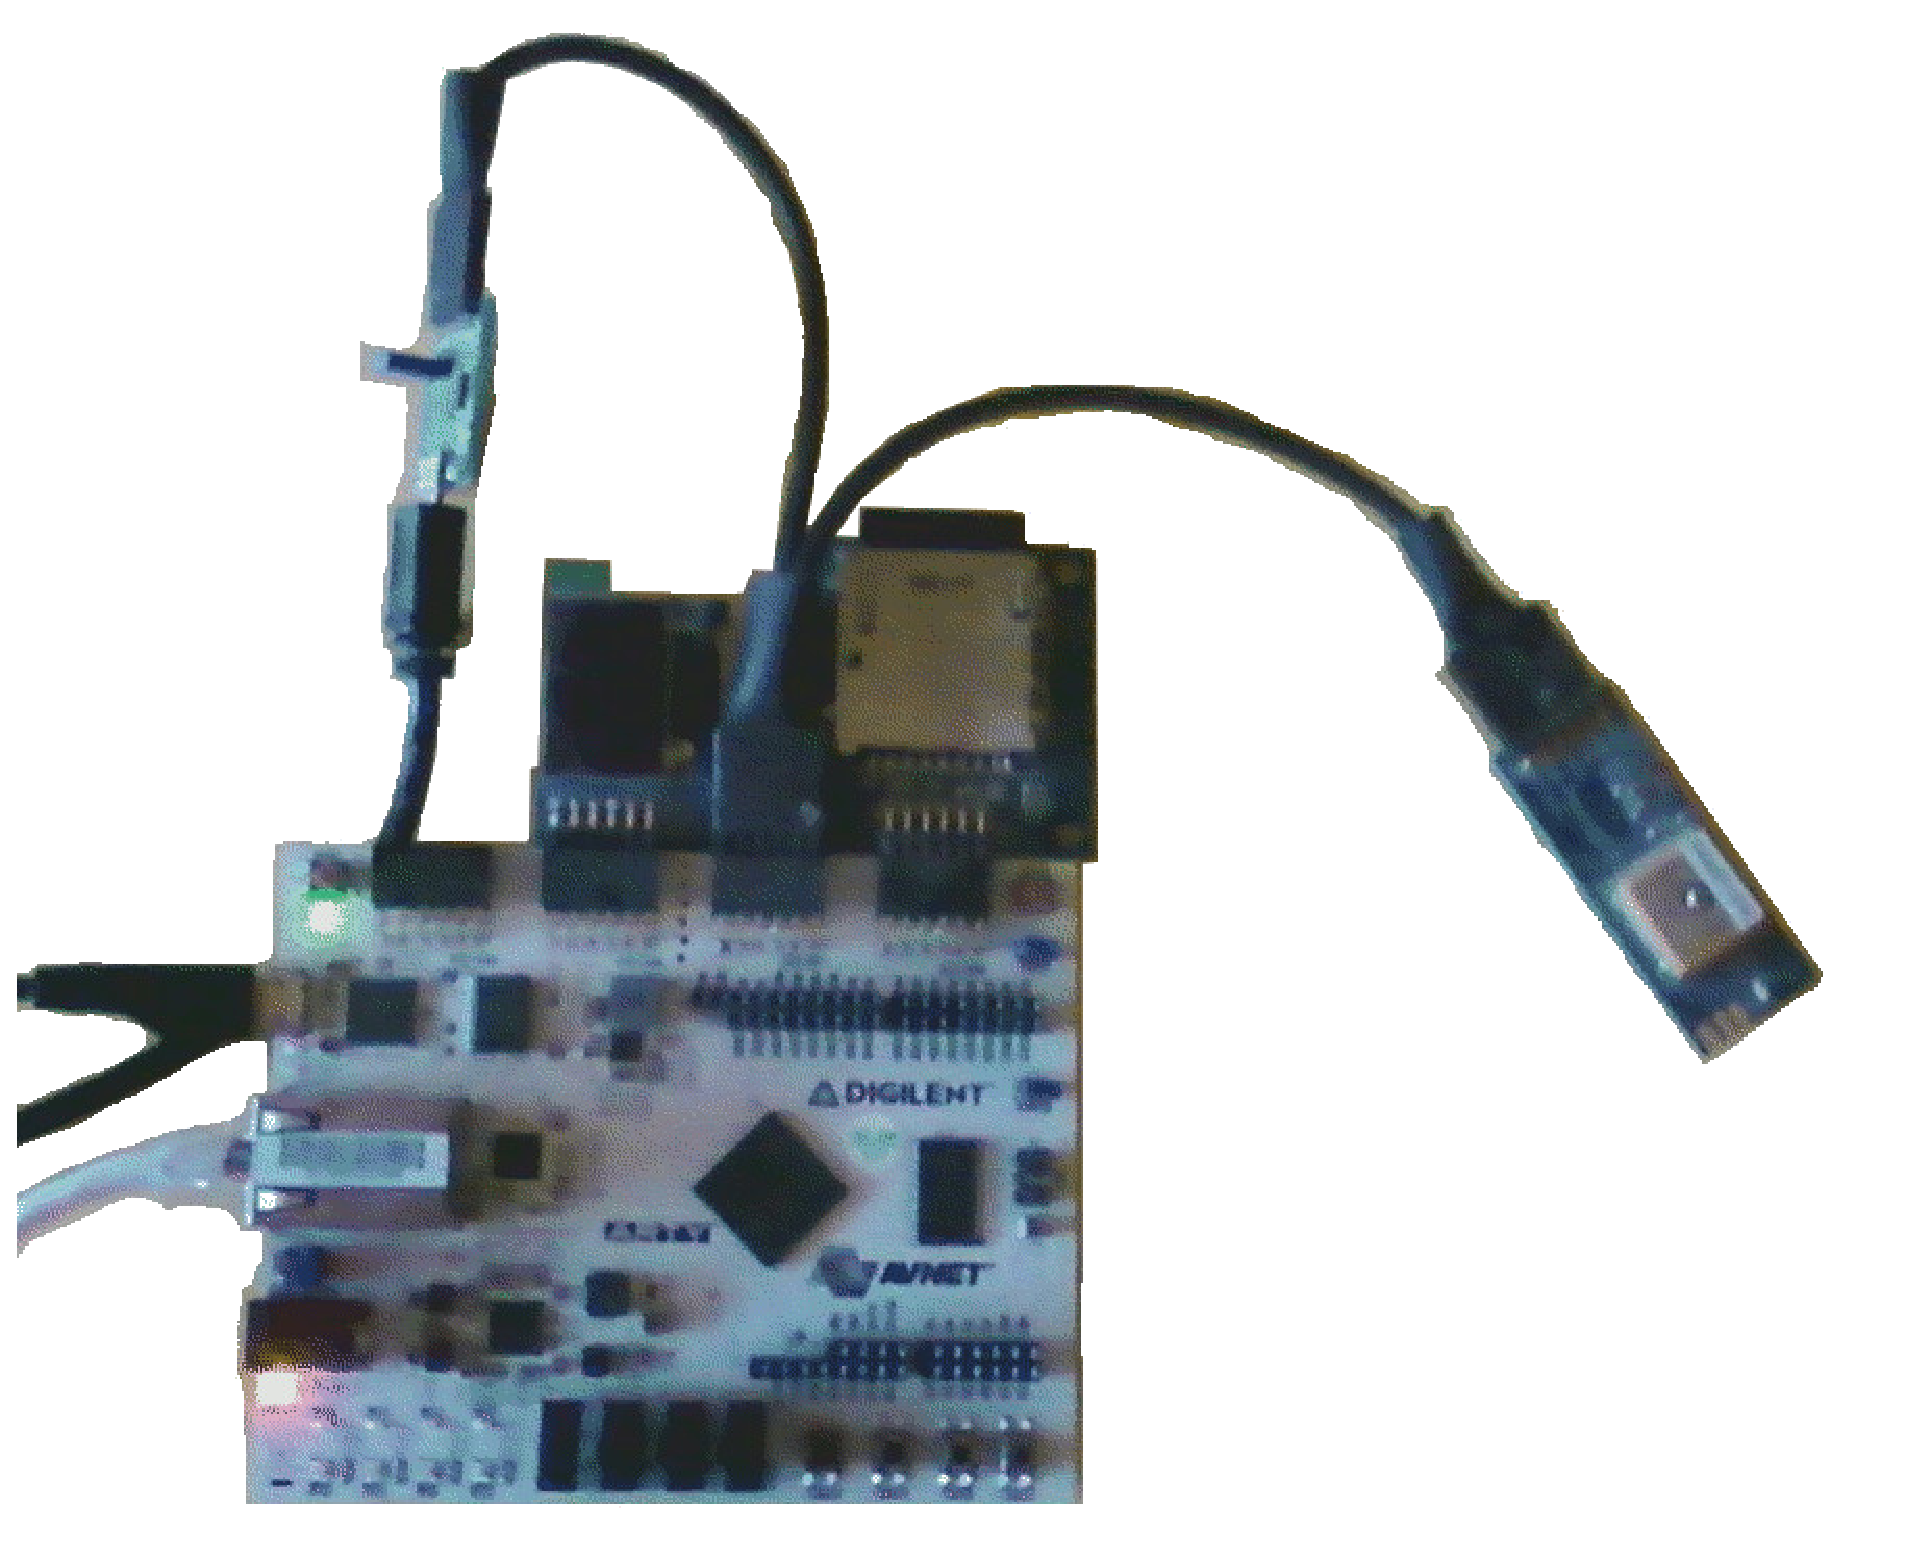
\includegraphics[width=4in]{../gfx/openarty.eps}
\caption{Showing how the PMods are Connected}\label{fig:pmod-pic}
\end{center}\end{figure}
In this example, the PModOLED is connected to PMod port JB, and the PModSD is
connected to PMod port JD.  Both the PModGPS and the PModUSBUART are both
connected to port JC, with the GPS connected on top and the USBUART on the
bottom.

\section{Testing the peripherals}
OpenArty has been designed so that all of the peripherals live on a 
memory--mapped wishbone bus.  This bus can be accessed, either by the ZipCPU
or by the host controller.  Because of this model, peripherals may be tested
and known to work before the CPU is ever turned on.  Two programs make this
possible: netuart and wbregs.  Other programs may be built upon this model,
as long as they access the bus using the interface outlined in devbus.h.

Of the two programs, netuart simply turns the USB serial port interface of
the device into a TCP/IP interface.  Netuart takes one argument, the 
name of the serial port device which the Arty USB driver has created.  In
my case, this tends to be /dev/ttyUSB1, although it has been known to change
from time to time:

\begin{lstlisting}[language=bash]
% netuart /dev/ttyUSB1
\end{lstlisting} 

All of the other board support files connect to the TCP/IP port generated
by netuart.  The port.h file is a compiled-in file, outlining where this
port can be found.  By default, netuart listens to port {\tt 6510} on
{\tt localhost}, but it can be configured to listen to any port.  The other
board support files will try to connect to netuart at the host and port
listed in port.h.  Hence, if properly configured, you should be able to 
access your Arty to command it, configure it, reload it, etc., from anywhere
you have internet access--in my case, from anywhere in the house.

Once you run netuart, you should then be able to watch, as a part of the
standard output stream of netuart, all of the interaction with the board.
While this may be useful for debugging, it's not all that legible to the
user.   Lines that start with \hbox{``\#''} are lines from the device that are not
going to any client.  A common line you will see is \hbox{``\# 0''}.  This is
just the device saying that its command capability is idle.  Lines that start
with \hbox{``< ''} are commands going to the device, and lines starting with
\hbox{``> ''} are responses from the core.  So, at this point, run netuart and
wait a couple of seconds.  If you do not see a \hbox{``\# 0''} line, then try a
different serial port, check that your core is properly configured, etc.  Once
you do see a \hbox{``\# 0''} line, then you are ready for the next step.

The easiest way to test the peripherals is via the wbregs command.  This
command is similar to the ancient peek and poke commands.  It takes one
or two arguments.  If given one argument, it reads from that address on the
bus.  If given two arguments, it writes the value of the second argument to
the bus location given by the first argument.  Hence one argument peeks
at the memory bus, two arguments pokes a value onto the memory bus.

Perhaps an example will help.  At this point, try typing:

\begin{lstlisting}[language=bash]
% wbregs version
\end{lstlisting}

This should return and print a 32-bit hexadecimal value to your screen,
indicating the date of when you last ran make in the root directory before
building and installing your configuration into the device.  This can be
very useful to know what configuration you are running, and whether or not
you have made the changes you thought you had made.

You may have noticed that wbregs read from address 0x0100, but did so by name.
Most of the peripherals have names for their addresses.  The C language
names for these addresses can be found in regdefs.h, and a mapping to 
wbregs address names can be found in regdefs.cpp.

Shall we try another?  Let's try adjusting the LEDs.  To turn all the LEDs off, 
\begin{lstlisting}[language=bash]
% wbregs leds 0x0f0
\end{lstlisting}
To turn them all back on again,
\begin{lstlisting}[language=bash]
% wbregs leds 0x0ff
\end{lstlisting}
To turn the low order LED off without changing any others, write
\begin{lstlisting}[language=bash]
% wbregs leds 0x010
\end{lstlisting}

Having fun?  Try running the program startupex.sh from the sw directory.
This will set some LEDs and Color LEDs in a fun, startup--looking, pattern.

Ready to test the UART?   Using minicom, connect to the PModUSBUART.  It 
should also be connected to a /dev/ttyUSBx serial port device.  If you aren't
sure, start minicom with:
\begin{lstlisting}[language=bash]
% minicom -D /dev/ttyUSB2
\end{lstlisting}
Then, configure minicom to use 115,200 Baud, 8-data bits, one stop bit, and
no parity. 

Once you've done that, we can test it by sending a character across the UART
port:
\begin{lstlisting}[language=bash]
% wbregs tx 90
\end{lstlisting}
This should send a `Z' over the UART port.  Did you see a `Z' in minicom?
If not, did you set the baud rate right?  The UART is supposed to be set
for 115,200 Baud, 8N1 by default.  If not, you can set it to that by writing
wbregs setup 705.  The 705 comes from the clock rate, in Hz, divided by 
115200.  By leaving other higher order bits at zero, this becomes the default
baud rate of an 8N1 serial port channel.

Another fun program to run is {\tt netsetup}.  This program takes no arguments,
and just reads and decodes the network registers via the MDIO port.  The
decoded result will be sent to the screen.

\section{Subsequent Core Updates}
The board support file {\tt wbprogram} can be used to write .bit or .bin
files to the flash, so that the core can be updated once an initial core
is installed and running. 
Although wbprogram expects the filename to end in either '.bit' or '.bin',
this is primarily to keep a user from doing something they don't intend to
do.

The basic usage of the wbprogram command is:
\begin{lstlisting}[language=bash]
% wbprogram [@address] file
\end{lstlisting}
wbprogram then copies the file to the flash, starting at the Arty address
of {\tt @address}.  If no address is given, wbprogram writes the file at the 
beginning of flash.

An example of how to do this can be found in the {\tt program.sh}.
{\tt program.sh} places the new configuration file into the alternate
configuration location.  (An alternate script, zprog.sh, places the new
configuration at the beginning of the flash, where the FPGA loader will look
for it upon power up.)  Once {\tt program.sh} places the new configuration
into flash, it then commands the FPGA via the ICAPE2 interface and an IPROG
command to reconfigure itself using this new configuration.  As a result, this
can be used to load subsequent configurations into the FLASH.

\section{Building the ZipCPU tool-chain}
At this point, you should have some confidence that your configuration and
hardware are working.  Therefore, let's transition to getting the ZipCPU
on the hardware up and running. 
To do this, we'll start with getting a copy
of the ZipCPU toolchain and building it.  Pick a directory to work in, and
then issue:
\begin{lstlisting}[language=bash]
% git clone https://github.com/ZipCPU/zipcpu
\end{lstlisting}
to get a copy of the ZipCPU project, together with toolchain.  You'll also
need to double check that you have the pre-requisite packages to build this
tool chain, so on an Ubuntu~14 machine you would issue:
\begin{lstlisting}[language=bash]
% sudo apt-get install flex bison libbison-dev
% sudo apt-get install libgmp10 libgmp-dev libmpfr-dev libmpc-dev libelf-dev
% sudo apt-get install libisl-dev
\end{lstlisting}
Once these are all in place, you can then switch to the master ZipCPU
directory and type,
\begin{lstlisting}[language=bash]
% cd zipcpu; make
\end{lstlisting}
(you may need to issue the make command a couple of times \ldots)

This will build the GCC compiler for the ZipCPU from source.  
It will also install this new compiler into the zipcpu/sw/install/cross-tools.
This new compiler will be called zip-gcc.

This will also build a copy of the binutils programs for the ZipCPU.  These
include the assembler, {\tt zip-gas}, linker, {\tt zip-ld}, disassembler,
{\tt zip-objdump}, and many more useful programs.

The next step to using this toolchain is to place it into your path.
\begin{lstlisting}[language=bash]
% export PATH=$PATH:$PWD/zipcpu/install/cross-tools/bin
\end{lstlisting}
Once the toolchain is in your path,
\begin{lstlisting}[language=bash]
% which zip-gcc
/home/.../zipcpu/sw/install/cross-tools/bin/zip-gcc
\end{lstlisting}
should return the location of where this toolchain exists in your path.

\section{Building your first ZipCPU program}
Several example programs for the OpenArty project can be found in the
{\tt sw/board} directory.  These can be used to test various peripherals from
the perspective of the CPU itself.

As a test of the build process, a good first progam to build would be 
{\tt exstartup}.  This program is very similar to the {\tt startupex.sh} shell
script you tried earlier.  It simply plays with the color LEDs and some
on board timers.   Once that is finished, it goes into a loop controlling
both the normal and the color LEDs based upon the button state and the switch
settings.

To build {\tt exstartup}, simply type {\tt make exstartup} from the 
{\tt sw/board} directory of the {\tt openarty} project.  (Don't forget to
include the ZipCPU toolchain into your path before you do this!)

\section{Loading a program}
Now that you have built your {\tt exstartup} program, it's time to load it
onto the board and start it up.  The {\tt zipload} program can be used to
do this.  {\tt zipload} can be found in the sw/host directory.  To load a
ZipCPU program into the Arty, just type {\tt zipload} and the program name,
such as {\tt exstartup} in this case.  To start the program immediately
after loading it, pass the `-r' option to {\tt zipload}.  In our case, you
would type:
\begin{lstlisting}[language=bash]
% zipload -r exstartup
\end{lstlisting}

Hopefully, you can see the {\tt exstartup} program now toggling the LED's.
Once the initial display stops, you can adjust the switches and press buttons
to see how that affects the result.

If you wish to restart the {\tt exstartup} program, or indeed to run another
program, you can just run {\tt zipload} again with the new program name.  This
will halt the previous program, and then load the new one into memory.  As 
before, if you use the `-r' option, the program will be started automatically.

\section{Some other test programs}
If you have the PModUSBUART, you might wish to try running a ``Hello, World''
program.  This can be found in the hello.c file.  It prints ``Hello, World''
to the PModUSBUART once every ten seconds.  Had enough of it?  You can stop
the CPU by typing {\tt wbregs cpu 0x0400}.  This sends a halt command to the
debug register of the ZipCPU.  More information about this debug register, and
other things that can be done via the debug register, can be found in the
ZipCPU specification.

If you have both the PModUSBUART as well as the PModGPS, the {\tt gpsdump.c}
program can be used to forward the NMEA stream from the GPS to the USBUART. 
This should give you some confidence that the PModGPS is working.

As a third test, {\tt oledtest.c} will initialize the OLEDrgb device and cause
it to display one of two images in an alternating fashion.

\chapter{Architecture}\label{ch:architecture}
My philosophy in peripherals is to keep them simple.  If there is a default
mode on the peripheral, setting that mode should not require turning any bits
on.  If a peripheral encounters an error condition, a bit may be turned on to
indicate this fact, otherwise status bits will be left in the off position.

\subsection{Bus Structure}
The OpenArty project contains four bus masters, three of them within the CPU.
These masters are the instruction fetch unit, the data read/write unit,
and the direct memory access peripheral within the ZipCPU, as well as an 
external debug port which can be commanded from over the main UART port
connecting the Arty to its host.  

There is also a second minor peripheral bus located within the ZipCPU
ZipSystem.  This bus provides access to a number of peripherals within the
ZipSystem, such as timers, counters, and the direct memory access controller.
This bus will also be used to configure the memory management unit once
integrated.  This bus is only visible to the CPU, and located starting at
address {\tt 0xc0000000}.

The ZipCPU debug port is also available on the bus.  This port, however, is
only visible to the external debug port.  It can be found at address
{\tt 0x08000000} for the control register, and {\tt 0x08000001} for the
data register.

Once the MMU has been integrated, it will be placed between the instruction
fetch unit, data read/write unit, and the rest of the peripheral bus.

The actual bus chosen for this design is the Wishbone Bus, based upon the
pipeline mode defined in the B4 specification.  All optional wires required
by this bus structure have been removed, such as the tag lines, the cycle
type identifier, the burst type, and so forth.  This was done to simplify
the logic within the core.

However, because of the complicated bus structure--particularly because of the
number of masters and slaves on the bus and the speed for which the bus is
defined, there are a number of delays and arbiters placed on the bus.  As a
result, the stall wire which is supposed to be depend upon combinational logic
only, has been registered at a number of locations.  What this means is that
there are a variety of delays as commands propagate through the bus structure.
Most of these are variable, in that they can be turned on or off at build time,
or even that the stall line may (or may not) be registered as configured.

All interactions between bus masters and any peripherals passes through the
interconnect, located in {\tt busmaster.v}.  This interconnect divides the
slaves into separate groups.  The first group of slaves are those for which the
bus is supposed to provide fast access to.  These are the DDR3 SDRAM, the
flash, the block RAM, and the network.  The next group of slaves will have their
acknowledgements delayed by an additional clock.  The final group of slaves
are those single register slaves whose results may be known ahead of any read,
and who only require one clock to access.  These are grouped together and
controlled from within {\tt fastio.v}.

Further information about the Wishbone bus structure found within this core
can be found either on the Wishbone datasheet (Ch.~\ref{ch:wishbone}), or in
the memory map table in the Registers chapter (Ch.~\ref{ch:registers}).

\subsection{DDR3 SDRAM}

{\em It is the intention of this project to use a completely open source
DDR3 SDRAM controller.  While the controller has been written, it has yet to
be successfully connected to the physical pins of the port.  Until that time,
the design is running using a Wishbone to AXI bus bridge.  Memory may still
be read or written, after an initial pipeline delay of roughly 27~clocks per
access, at one access per clock.}

{\em The open source SDRAM controller should be able to achieve a delay closer
to 9~clocks per access--once I figure out how to connect it to the PHY.}

\subsection{Flash}
\subsection{Block RAM}

The block RAM on this board has been arranged into one 32kW section.
Programs that use block RAM will run fastest using the block RAM, both for
instructions as well as for memory.  

\subsection{Ethernet}

The ether net controller has been split into three parts.  The first part is
an area of packet memory.  This part is simple: it acts like memory.  The
receive memory is read only, whereas the transmit memory is both read and
write.  Packets received by the controller will be found in the receive memory,
packets transmitted must be in the transmit area of memory.  The octets
may be found in memory with the first octet in the most significant byte.
This is the easy part.

The format of the packets within this memory is a touch more interesting.
With no options turned on, the first 6~bytes are the destination MAC
address, the next 6~bytes will be the source MAC address, and the {\em next
4~bytes} will be the EtherType repeated twice.  This was done to align the
packet, and particularly the IP header, onto word boundaries.  If the hardware
CRC has been turned off, the packet must contain its own CRC as well as
ensuring that it has a minimum packet length (64 octets) when including that
CRC.

With all options turned on, however, things are a touch simpler.  The first
two words of the packet contain the destination MAC (for a transmit packet)
or the source MAC (for a received packet), followed by the two--octet
EtherType.  At this point the packet is word--aligned prior to the IP header.
Since broadcast packets are sent to a special destination MAC other than
our own, a flag in the command register will indicate this fact.


The second part of the controller is the MDIO interface.  This follows from
the specification, and can be used to toggle the LED's on the ethernet,
to force the ethernet into a particular mode, either 10M or 100M, to control
auto--negotiation of the speed, and more.  Reads or writes to MDIO memory
addresses will command reads or writes via the MDIO port from the FPGA to the
ethernet PHY.  As the PHY can only handle 16--bit words, only 16~bits will
ever be transferred as a result of any read/write command, the top 16~bits
are automatically set to zero.  Further details of this capability may be
found within the specification for the chip.

The MDIO interface may be ignored.  If ignored, the defaults within the
interface will naturally set up the network connection in full duplex mode (if
your hardware supports it), at the highest speed the network will support.  
However, if you ignore this interface you may not know what problems you are
suffering from this interface, if any.  The {\tt netsetup} program has been
provided, among the host software, to help diagnose how the various MDIO
registers have been set, and what the status is that is being reported from
the PHY.

The third part of the controller is the packet command interface.  This
consists of two command registers, one for reading and one for writing.
Before doing anything with the network, it must first be taken out of 
reset.  According to the specification for the network chip, this must
happen a minimum of one second after power up.  This may be done by simply
writing to the transmit command register with the reset bit turned off.

To send a packet, simply write the number of octets in the packet to the
transmit control register and set the GO bit ({\tt 0x04000}).  Other bits
in this control register can be used to turn off the hardware MAC generation
(and removal upon receive), the hardware CRC checking, and/or the hardware
IP header checksum validation (but not generation).  The GO bit will remain
high while the packet is being sent, and only transition to low once the
packet is away.  While the packet is being sent, a zero may be written to the
command register to cancel the packet--although this is not recommended.

Packets are automatically received without intervention.  Once a packet has been
received, the available bit will be set in the receive command register and
a receive packet interrupt will be generated.  The ethernet port will then
halt/stall until a user has reset the receive interface so that it may
receive the next packet.  Without clearing this interface, the receive port
will not accept further packets.  Other status bits in this interface are
used to indicate whether packets have been missed (because the interface was
busy), or thrown out due to some error such as a CRC error or a more general
error.\footnote{It should be possible to extend this interface so that further
packets may be read as long as the memory isn't yet full.  This is left as an
exercise to others.}

\subsection{SD Card}
\subsection{GPS Tracking}
\subsection{Configuration port}

The registers associated with the ICAPE2 port have been made accessible
to the core via the {\tt wbicapetwo} core.  More information about the meaning
of these registers can be found in Xilinx's ``7--Series FPGAs Configuration
User's Guide''.  

Testing with the OpenArty board has tended to focus on the warmboot capability.
Using this capability, a user is able to command the FPGA to reload its
configuration.  In support of this, two configuration areas have been 
defined within memory.  The first is the default configuration, found at
the beginning of the flash.  This configuration is sometimes called the ``golden
configuration'' within Xilinx's documentation because it is the configuration
that the Xilinx device will always start up from after a power on reset.  On
the OpenArty, a second configuration may immediately follow the first in flash. 
Commanding the FPGA to reload it's configuration is as simple as
setting the WBSTAR (warm boot start address) register to the location of the
new configuration within the flash, and then writing a 15 (a.k.a. IPROG)
to the FPGA command register (offset 4 from the beginning of the ICAPE2
addresses).  Examples of doing this are found in the 
{\tt sw/host/zprog.sh} and {\tt sw/host/program.sh} scripts.  The former
programs the default configuration and then switches to it, 

This configuration capability makes it possible for a user to 1) reprogram
the flash with an experimental configuration in the second configuration
location, and 2) test the configuration without actually touching the board. 
If the configuration doesn't work well enough to be communicated with, the
board may simply be powered down and it will come back up with the initial
or golden configuration.  If the golden configuration ever gets corrupted,
or loaded with a configuration that will not work, then the user will need to
reload the FPGA from the JTAG port.

\subsection{OLED}
\subsection{Real Time Clock}

The Arty board contains a real time clock core together with a companion
real time date/calendar core.  The clock core itself contains not only current
time, but also a stopwatch, seconds timer, and alarm.  The real time date core
can be used to maintain the current date.  The real--time clock core uses the
GPS PPS output, as schooled by the GPS tracking circuit, in order to synchronize
their subsecond timing to the GPS itself.  Further, the real--time clock core
then creates a synchronization wire for the real--time date core.

Neither of these cores exports its subsecond precision to the rest of the
design.  This must be done using either the internal GPS tracking wires, or
by reading the time information from the tracking test bench.

\subsection{LEDs}

The Arty board contains two sets of LEDs: a plain set of LEDs, and a colored
set of LEDs.

The plain set of LEDs is controlled simply from the LED register.  This register
can be used to turn these LEDs on and off, either individually or as a whole.
It has been designed for atomic access, so only one write to this register
is necessary to set any particular LED.

The color LEDs are slightly different.  Each color LED is supported by its
own register, which controls three pulse width modulation controllers.  Three
groups of eight bits within the color LED register control the PWM thresholds,
first for red, then green, and then in the lowest bits for blue.  These are
used to turn on and off the various color components of the LEDs.  Using this
method, there are $2^{24}$ different colors each of these LEDs may be set
to.  

\subsection{Buttons}
\subsection{Switches}
\subsection{Startup counter}

A startup counter has been placed into the basic peripheral I/O area.  This 
counter simply counts the clocks since startup.  Upon rollover, the high
order bit remains set.  This can be used to sequence the start up of components
within the design if so desired.

\subsection{GPS UART}
The GPS UART, debug control UART, as well as the auxilliary UART, are all
based upon the same underlying UART IP core, sometimes known as the WBUART32
core.  The setup register is defined within the documentation for that core,
and provides for a large baud rate selection, 5-8 data bits, 1-2 stop bits,
and several parity choices.  Within OpenArty, the GPS core is initialized
to 9.6~kBaud, 8 data bits, no parity, and one stop bit.  

When a value is ready to be read from the GPS uart, the GPS interrupt line
will go high.  Once read, and only when read, will this interrupt line reset.
If the read is successful, only bits within the bottom eight will be set.
If a read is attempted when there is no data, when the UART is in a reset
condition, or when there has been a framing or parity error (were parity
to be turned on), the upper bits of the UART port will be set.

In a like manner, the GPS device can be written to.  Certain strings, if sent
to the UART, can be used to change the UARTs baud rate, its serial port
settings, or even its reporting interval.  As with the read port, the transmit
port will interrupt the CPU when it is idle.  Writing a character to this
port will reset the interrupt.  Setting bits other than the bottom eight may
result in a break condition being set on this port as well.

Interacting with a controller can therefore be somewhat tricky.  The
interrupt controller will trigger whenever the port is ready to be read from,
and will re--trigger every clock until the port has been read from.  At this
point, the interrupt controller may be reset.  If this is an auxilliary
interrupt controller, such as the bus interrupt controller or the ZipSystem's
auxiliary controller, the auxiliary controller will then need to be reset,
and the bit in the primary controller associated with the auxiliary controller
as well.  It is for this reason that the UARTs have been placed on the
primary controller only.

It should also be possible to use the DMA to read from (or write to) either
UART port.

\subsection{Auxilliary UART}

The Auxilliary UART has roughly the same structure as the GPS UART, save that
it's default configuration is for a 115,200~Baud configuration with 8~data bits,
no stop bits, and no parity.  Reads, writes, and interrupts are treated in
the same fashion.

\subsection{GPIO}

A General Purpose I/O controller has been placed within the design as well.
This controller can handle 16--generic input wires, and set 16--generic output
wires.  A single register is used to read both input and output wire values,
as well as to set output values when written to. 

However, to use this controller, you will need to manually configure it
(i.e.~change the Verilog source) within the core, in order to wire the various
GPIO values up to a device of interest.  This was done for the simple reason
that wiring anything new up to the controller will require Verilog changes
anyway.  For this reason, the controller has no way of setting wires to high
impedence, or pulling them up or down.  Such control may be done within the
top level design if necessary.

This controller will set an interrupt if ever any of the input wires within
it are changed.  The interrupt may be cleared in the interrupt controller.

\subsection{Linker Script}

A linker script has been created to capture the memory structure needed by
a program.  This script may be found in {\tt sw/board/arty.ld}.  It is a
sample script, using it is not required.

The script defines three types of memory to the linker: flash, block RAM, and
SDRAM.  Programs using this script will naturally start in flash (acting as
a ROM memory).  A bootloader must then be used to copy, from flash, those
sections of the program that are to be placed in block RAM or SDRAM into
their particular memory locations.

The block RAM locations are reserved for the user kernel, and specifically for
any part of the code in the {\tt .kernel} section.  C attributes, or assembly
{\tt .section} commands, must be used to place items within this section.
A final symbol within this section, {\_top\_of\_stack}, is used so that the
initial boot loader knows what to set the initial kernel stack to.

The rest of the initial program's memory is placed into
SDRAM.\footnote{Hopefully,
I'll get a data cache running on the ZipCPU to speed this up.}  At the end,
a {\tt \_top\_of\_heap} symbol is set to reference the final location in the
setup.  This symbol can then be used as a starting point for a memory allocator.

An example bootloader is provided in {\tt sw/board} that can be linked with
any (bare metal, supervisor) program in order to properly load it into memory.

\chapter{Software}
\section{Directory Structure}
\section{Zip CPU Tool Chain}
\section{Bench Test Software}
\section{Host Software}
\begin{itemize}
\item {\tt readflash}: As I am loathe to remove anything from
	a device that came factory installed, the
	{\tt readflash} program reads the original installed
	configuration from the flash and dumps it to a file.

\item {\tt wbregs}: This program offers a capability very similar to the 
	PEEK and POKE capability Apple user's may remember from before the
	days of Macintosh.  {\tt wbregs <address>} will read from the
	Wishbone bus the value at the given address.  Likewise
	{\tt wbregs <address> <value>} will write the given value into the
	given address.  While both address and value have the semantics of
	numbers acceptable to {\tt strtoul()}, the address can also be a named
	address.  Supported names can be found in {\tt regdefs.cpp}, and their
	register mapping in {\tt regdefs.h}.
\item {\tt ziprun}:
\item {\tt zipload}:
\end{itemize}

\section{Zip CPU Programs}
\begin{itemize}
\item {\tt ntpserver}:
\item {\tt goldenstart}:
\end{itemize}
\section{ZipOS}
\subsection{System Calls}
\begin{itemize}
\item {\tt int wait(unsigned event\_mask, int timeout)}
\item {\tt int clear(unsigned event\_mask, int timeout)}
\item {\tt void post(unsigned event\_mask)}
\item {\tt void yield(void) }
\item {\tt int read(int fid, void *buf, int len)}
\item {\tt int write(int fid, void *buf, int len)}
\item {\tt unsigned time(void) }
% \item SEMGET
% \item SEMPUT
\item {\tt void *malloc(void)}
\item {\tt void free(void *buf)}
% \item FORK
% \item opendir
% \item EXEC
% \item OPEN
\end{itemize}
\subsection{Scheduler}

\chapter{Operation}\label{ch:operation}

\chapter{Registers}\label{ch:registers}
There are several address regions within the {\tt OpenArty}, as shown in
Tbl.~\ref{tbl:memregions}.
\begin{table}[htbp]
\begin{center}\begin{tabular}{|p{2.25in}|p{0.6in}|p{0.35in}|p{2.0in}|}\hline
\rowcolor[gray]{0.85} Binary Address & \multicolumn{1}{c|}{Base} & \multicolumn{1}{c|}{Size} & Purpose \\\hline\hline
\scalebox{0.8}{\tt 00 0000 0000 0000 0000 0100 0xxx xx--} & \scalebox{0.9}{\tt 0x00000400} & \hfill 128 & Peripheral I/O Control \\\hline
\scalebox{0.8}{\tt 00 0000 0000 0000 0000 0100 100y yx--} & \scalebox{0.9}{\tt 0x00000480} & \hfill 32& Debug scope control\\\hline
\scalebox{0.8}{\tt 00 0000 0000 0000 0000 0100 1010 xx--} & \scalebox{0.9}{\tt 0x000004a0} & \hfill 16 & RTC control\\\hline
\scalebox{0.8}{\tt 00 0000 0000 0000 0000 0100 1011 xx--} & \scalebox{0.9}{\tt 0x000004b0} & \hfill 16 & OLEDrgb control\\\hline
\scalebox{0.8}{\tt 00 0000 0000 0000 0000 0100 1100 xx--} & \scalebox{0.9}{\tt 0x000004c0} & \hfill 16 & AUX UART\\\hline
\scalebox{0.8}{\tt 00 0000 0000 0000 0000 0100 1101 xx--} & \scalebox{0.9}{\tt 0x000004d0} & \hfill 16 & GPS UART\\\hline
\scalebox{0.8}{\tt 00 0000 0000 0000 0000 0100 1110 xx--} & \scalebox{0.9}{\tt 0x000004e0} & \hfill 16 & SDCard controller\\\hline
\scalebox{0.8}{\tt 00 0000 0000 0000 0000 0101 0000 xx--} & \scalebox{0.9}{\tt 0x00000500} & \hfill 16 & GPS Clock loop control\\\hline
%\scalebox{0.8}{\tt 00 0000 0000 0000 0001 0101 0001 ----} & \scalebox{0.9}{\tt 0x00000148} & \hfill 16 & {\em Unused}\\\hline
\scalebox{0.8}{\tt 00 0000 0000 0000 0000 0101 001x xx--} & \scalebox{0.9}{\tt 0x00000520} & \hfill 32 & GPS Testbench\\\hline
\scalebox{0.8}{\tt 00 0000 0000 0000 0000 0101 010x xx--} & \scalebox{0.9}{\tt 0x00000540} & \hfill 32 & Network packet interface\\\hline
%\scalebox{0.8}{\tt 00 0000 0000 0000 0001 0101 011- ----} & \scalebox{0.9}{\tt 0x00000150} & \hfill 16 & {\em Unused}\\\hline
\scalebox{0.8}{\tt 00 0000 0000 0000 0000 0101 1xxx xx--} & \scalebox{0.9}{\tt 0x00000580} & \hfill 128 & Ethernet MIO configuration\\\hline
\scalebox{0.8}{\tt 00 0000 0000 0000 0000 0110 0xxx xx--} & \scalebox{0.9}{\tt 0x00000600} & \hfill 128 & Extended Flash Control Port\\\hline
\scalebox{0.8}{\tt 00 0000 0000 0000 0000 0110 1xxx xx--} & \scalebox{0.9}{\tt 0x00000680} & \hfill 128 & ICAPE2 Configuration Port\\\hline
%\scalebox{0.8}{\tt 00 0000 0000 0000 0000 0111 ---- ----} & \scalebox{0.9}{\tt 0x00000150} & \hfill 16 & {\em Unused}\\\hline
%\scalebox{0.8}{\tt 00 0000 0000 0000 0000 1--- ---- ----} & \scalebox{0.9}{\tt 0x00000150} & \hfill 16 & {\em Unused}\\\hline
%\scalebox{0.8}{\tt 00 0000 0000 0000 0001 ---- ---- ----} & \scalebox{0.9}{\tt 0x00000150} & \hfill 16 & {\em Unused}\\\hline
\scalebox{0.8}{\tt 00 0000 0000 0000 0010 xxxx xxxx xxxx} & \scalebox{0.9}{\tt 0x00002000} & \hfill 4k & Ethernet RX Buffer\\\hline
\scalebox{0.8}{\tt 00 0000 0000 0000 0011 xxxx xxxx xxxx} & \scalebox{0.9}{\tt 0x00003000} & \hfill 4k & Ethernet TX Buffer\\\hline
\scalebox{0.8}{\tt 00 0000 0000 001x xxxx xxxx xxxx xxxx} & \scalebox{0.9}{\tt 0x00020000} & \hfill 128k & On-chip Block RAM\\\hline
\scalebox{0.8}{\tt 00 0001 xxxx xxxx xxxx xxxx xxxx xxxx} & \scalebox{0.9}{\tt 0x01000000} & \hfill 16M & QuadSPI Flash\\\hline
\scalebox{0.8}{\tt 00 0001 0000 0000 0000 0000 0000 0000} & \scalebox{0.9}{\tt 0x01000000} & & Configuration Start\\\hline
\scalebox{0.8}{\tt 00 0001 0100 0111 0000 0000 0000 0000} & \scalebox{0.9}{\tt 0x011c0000} & & Alternate Configuration\\\hline
\scalebox{0.8}{\tt 00 0001 0000 1110 0000 0000 0000 0000} & \scalebox{0.9}{\tt 0x01380000} & & CPU Reset Address\\\hline
\scalebox{0.8}{\tt 01 xxxx xxxx xxxx xxxx xxxx xxxx xxxx} & \scalebox{0.9}{\tt 0x10000000} & \hfill 256M & DDR3 SDRAM\\\hline
\scalebox{0.8}{\tt 10 0000 0000 0000 0000 0000 0000 0x00} & \scalebox{0.9}{\tt 0x20000000} & \hfill 8 & ZipCPU debug control port---only visible to debug WB master\\\hline
\end{tabular}
\caption{Address Regions}\label{tbl:memregions}
\end{center}\end{table}
These address regions include both read and write memory regions, such as the
block RAM, the SDRAM, and the Ethernet TX buffer, as well as read only memory
regions, such as the flash memory and the Ethernet RX buffer, as well as a 
whole lot of memory mapped peripherals.  The purpose of this chapter will be
to describe how these memory mapped peripherals are organized, as well as
the specific details of how they may be used.

This address map information is also contained in a couple other locations.
First, {\tt sw/host/regdefs.h} maps all of the OpenArty registers to 
C++ names, whereas {\tt sw/host/regdefs.cpp} maps these C++ names to a more
human readable form which is used by {\tt wbregs}.  Second, these registers
are also given names as part of several various structures within 
{\tt sw/board/artyboard.h}.  And then, of course, they are also listed here.

\section{ZipSystem}
The ZipSystem wrapper around the ZipCPU provides access to roughly twenty
registers that are tightly integrated with the ZipCPU.  These registers are
shown in Tbl.~\ref{tbl:zipio}
\begin{table}[htbp]
\begin{center}\begin{tabular}{|p{0.9in}|p{0.35in}|p{2.5in}|}\hline
\rowcolor[gray]{0.85} Address & \multicolumn{1}{c|}{Size} & Purpose \\\hline\hline
\scalebox{0.9}{\tt 0xff000000} & 4 & Primary Zip PIC\\\hline
\scalebox{0.9}{\tt 0xff000004} & 4 & Watchdog Timer\\\hline
\scalebox{0.9}{\tt 0xff000008} & 4 & Bus Watchdog Timer\\\hline
\scalebox{0.9}{\tt 0xff00000c} & 4 & Alternate Zip PIC\\\hline
\scalebox{0.9}{\tt 0xff000010} & 4 & ZipTimer-A\\\hline
\scalebox{0.9}{\tt 0xff000014} & 4 & ZipTimer-B\\\hline
\scalebox{0.9}{\tt 0xff000018} & 4 & ZipTimer-C\\\hline
\scalebox{0.9}{\tt 0xff00001c} & 4 & ZipJiffies\\\hline
%
\scalebox{0.9}{\tt 0xff000020} & 4 & Master task counter\\\hline
\scalebox{0.9}{\tt 0xff000024} & 4 & Master prefetch stall counter\\\hline
\scalebox{0.9}{\tt 0xff000028} & 4 & Master memory stall counter\\\hline
\scalebox{0.9}{\tt 0xff00002c} & 4 & Master instruction counter\\\hline
\scalebox{0.9}{\tt 0xff000030} & 4 & User task counter\\\hline
\scalebox{0.9}{\tt 0xff000034} & 4 & User prefetch stall counter\\\hline
\scalebox{0.9}{\tt 0xff000038} & 4 & User memory stall counter\\\hline
\scalebox{0.9}{\tt 0xff00003c} & 4 & User instruction counter\\\hline
%
\scalebox{0.9}{\tt 0xff000040} & 4 & DMA command register\\\hline
\scalebox{0.9}{\tt 0xff000044} & 4 & DMA length\\\hline
\scalebox{0.9}{\tt 0xff000048} & 4 & DMA source address\\\hline
\scalebox{0.9}{\tt 0xff00004c} & 4 & DMA destination address\\\hline
%
\scalebox{0.9}{\tt 0xff000050} & 8 & {\em Reserved for MMU context register}\\\hline
\scalebox{0.9}{\tt 0xff8xxxxx} & ? & {\em Reserved for MMU TLB}\\\hline
\end{tabular}
\caption{ZipSystem Addresses}\label{tbl:zipio}
\end{center}\end{table}
and described in detail within the ZipCPU specification.

Unlike the rest of the address map, these registers are only visible to the
ZipCPU.  While many of them may be read via the debug port, in general accessing
these registers via the {\tt wbregs} command is not so straight forward.

\section{Peripheral I/O Control}
The first section of memory--mapped I/O for the ZipCPU is found near address
{\tt 0x100}.  These peripherals are specifically peripherals that can be
accessed without ever stalling the bus, and with a known and fixed (minimum)
delay.  Tbl.~\ref{tbl:ioregs}
\begin{table}[htbp]
\begin{center}\begin{reglist}
VERSION  &\scalebox{0.8}{\tt 0x0400} & 32 & R & Build date\\\hline
PIC      &\scalebox{0.8}{\tt 0x0404} & 32 & R/W & Bus Interrupt Controller \\\hline
BUSERR   &\scalebox{0.8}{\tt 0x0408} & 32 & R & Last Bus Error Address\\\hline
PWRCOUNT &\scalebox{0.8}{\tt 0x040c} & 32 & R & Ticks since startup (roughly)\\\hline
BTNSW    &\scalebox{0.8}{\tt 0x0410} & 32 & R/W & Button/Switch controller\\\hline
LEDCTRL  &\scalebox{0.8}{\tt 0x0414} & 32 & R/W & LED Controller \\\hline
RTCDATE  &\scalebox{0.8}{\tt 0x0418} & 32 & R/W & BCD Calendar Date\\\hline
GPIO     &\scalebox{0.8}{\tt 0x041c} & 32 & R/W & GPIO controller\\\hline
CLR-LEDx &\scalebox{0.8}{\tt 0x0420-c} & 32 & R/W & Color LED controller\\\hline
GPSSECS  &\scalebox{0.8}{\tt 0x0430} & 32 & R/W & {\em Reserved for a one-up seconds counter}\\\hline
GPSSUB   &\scalebox{0.8}{\tt 0x0414} & 32 & R/W & GPS PPS tracking subsecond info\\\hline
GPSSTEP  &\scalebox{0.8}{\tt 0x0418} & 32 & R/W & Current GPS step size, units TBD\\\hline
% Unused  &\scalebox{0.8}{\tt 0x041c--0x047f} & 32 & {\em Unused, writes ignored, returns zero upon read}\\\hline
% 0x010c-0x010f
\end{reglist}
% UARTRX   &\scalebox{0.8}{\tt 0x0430} & 32 & R/W & Aux UART receive byte\\\hline
% UARTTX   &\scalebox{0.8}{\tt 0x0434} & 32 & R/W & Aux UART transmit byte\\\hline
% GPSRX    &\scalebox{0.8}{\tt 0x0438} & 32 & R/W & GPS UART receive byte\\\hline
% GPSTX    &\scalebox{0.8}{\tt 0x0411} & 32 & R/W & GPS UART transmit byte\\\hline
% AUXSETUP &\scalebox{0.8}{\tt 0x0418} & 29 & R/W & Auxilliary UART config\\\hline
% GPSSETUP &\scalebox{0.8}{\tt 0x041c} & 29 & R/W & GPS UART config\\\hline
\caption{I/O Peripheral Registers}\label{tbl:ioregs}
\end{center}\end{table}
shows the addresses of these I/O peripherals included as part of OpenArty.
We'll walk through each of these peripherals in turn, describing how they work.

\subsection{Version}
One of the simpler peripherals on the board is the {\tt VERSION} peripheral.
This simple returns the date stamp found within {\tt rtl/builddate.v}.  This
stamp is updated any time a {\tt make} command is issued in the main OpenArty
project directory.  Reads from this address return this value, writes to this
address are ignored.

This peripheral is {\em very} useful, especially when trying to determine which
version of your configuration you are using, and whether or not the
configuration has been changed or updated as you had intended by loading a new
configuration, by writing a configuration to the flash and issuing an IPROG
command, etc.

\subsection{Interrupt Controller}
The OpenArty design maintains three interrupt controllers.  Two of them
(a primary and an auxiliary) are found within the ZipSystem, and the third is
located on the bus itself.  In terms of functionality, all three interrupt
controllers are the same, and documented in the ZipCPU specification.  Of
these, the primary interrupt controller for the
entire design is the primary interrupt controller within the ZipSystem.
This interrupt controller accepts as inputs, the output of the auxilliary
interrupt controller.
Hence, even though the CPU only supports a single interrupt line, by cascading
it with a second controller, many more interrupts can be supported.

The third interrupt controller is the bus interrupt controller.  While the
CPU can read and write this controller, the interrupt line from this controller
goes to the host interface.  If you see, as an example, an \hbox{``> 4''} in
your {\tt netuart} window, then you will know that OpenArty has sent an
interrupt to a waiting host program.  If what you saw instead was a
\hbox{``\# 4''}, then the interrupt was sent, but no one was listening.

The primary interrupt controller handles interrupts from the sources listed
in Tbl.~\ref{tbl:sys-ints}. 
\begin{table}[htbp]
\begin{center}\begin{tabular}{|p{1.0in}|c|r|p{3.00in}|}\hline
\rowcolor[gray]{0.85} Name & Bit Mask & DMAC ID &Description \\\hline\hline
SYS\_DMAC   & 0x0001 && The DMA controller is idle.\\\hline
SYS\_JIF    & 0x0002 & 1 & A Jiffies timer has expired.\\\hline
SYS\_TMC    & 0x0004 & 2 & Timer C has timed out.\\\hline
SYS\_TMB    & 0x0008 & 3 & Timer C has timed out.\\\hline
SYS\_TMA    & 0x0010 & 4 & Timer C has timed out.\\\hline
SYS\_AUX    & 0x0020 & 5 & The auxilliary interrupt controller sends an interrupt\\\hline
SYS\_PPS    & 0x0040 & 6 & An interrupt marking the top of the second\\\hline
SYS\_NETRX  & 0x0080 & 7 & A packet has been received via the network\\\hline
SYS\_NETTX  & 0x0100 & 8 & The network controller is idle, having sent its
			last packet\\\hline
SYS\_UARTRXF & 0x0200 &  9 & The receive UART FIFO is half-full\\\hline
SYS\_UARTTXF & 0x0400 & 10 & The transmit UART FIFO is less than half-full\\\hline
SYS\_GPSRXF  & 0x0800 & 11 & The GPS receive UART FIFO is half-full\\\hline
SYS\_GPSTXF  & 0x1000 & 12 & The GPS transmit UART FIFO is half-empty\\\hline
SYS\_BUS    & 0x2000 & 13 & The BUS interrupt controller sends an interrupt\\\hline
SYS\_OLED   & 0x4000 & 14 & The OLED port is idle\\\hline
\end{tabular}
\caption{Primary System Interrupts}\label{tbl:sys-ints}
\end{center}\end{table}
These interrupts are listed together with the
mask that would need to be used when referencing them to the interrupt
controller.  In a similar fashion, the auxilliary interrupt controller accepts
inputs from the sources listed in Tbl.~\ref{tbl:aux-ints}.  
\begin{table}[htbp]
\begin{center}\begin{tabular}{|p{0.9in}|c|r|p{3.00in}|}\hline
\rowcolor[gray]{0.85} Name & Bit Mask & DMAC ID &Description \\\hline\hline
AUX\_UIC & 0x0001 & 16 & The user instruction counter has overflowed.\\\hline
AUX\_UPC & 0x0002 & 17 & The user prefetch stall counter has overflowed.\\\hline
AUX\_UOC & 0x0004 & 18 & The user ops stall counter has overflowed.\\\hline
AUX\_UTC & 0x0008 & 19 & The user clock tick counter has overflowed.\\\hline
AUX\_MIC & 0x0010 & 20 & The supervisor instruction counter has overflowed.\\\hline
AUX\_MPC & 0x0020 & 21 & The supervisor prefetch stall counter has overflowed.\\\hline
AUX\_MOC & 0x0040 & 22 & The supervisor ops stall counter has overflowed.\\\hline
AUX\_MTC & 0x0080 & 23 & The supervisor clock tick counter has overflowed.\\\hline
%
AUX\_PPD    & 0x0100 & 24& True at midnight\\\hline
AUX\_UARTRX & 0x0200 & 25& A byte has been received from the AUX UART port and is ready to be read\\\hline
AUX\_UARTTX & 0x0400 & 26& There's room for another byte in the TXFIFO queue\\\hline
AUX\_GPSRX  & 0x0800 & 27& A byte has been received in the GPS UART interface, and is now ready to be read\\\hline
AUX\_GPSTX  & 0x1000 & 28& There's room in the GPS UART transmit FIFO for another byte\\\hline
\end{tabular}
\caption{Auxilliary System Interrupts}\label{tbl:aux-ints}
\end{center}\end{table}
These interrupt mask constants are also defined in {\tt sw/board/artyboard.h}
and {\tt sw/board/zipsys.h}.

Finally, the bus interrupt controller handles the interrupts from the sources
listed in Tbl.~\ref{tbl:bus-ints}.
\begin{table}[htbp]
\begin{center}\begin{tabular}{|p{0.9in}|c|p{3.75in}|}\hline
\rowcolor[gray]{0.85} Name & Bit Mask & Description \\\hline\hline
BUS\_BUTTON & 0x0001 & A Button has been pressed. \\\hline
BUS\_SWITCH & 0x0002 & The Scope has completed its collection\\\hline
BUS\_PPS    & 0x0004 & Top of the second\\\hline
BUS\_RTC    & 0x0008 & An alarm or timer has taken place (assuming the RTC
		is installed, and includes both alarm or timer)\\\hline
BUS\_NETRX & 0x0010 & A packet has been received via the network\\\hline
BUS\_NETTX & 0x0020 & The network controller is idle, having sent its
			last packet\\\hline
BUS\_UARTRX & 0x0040 & A character has been received via the UART\\\hline
BUS\_UARTTX & 0x0080 & The transmit UART is idle, and ready for its next
		character.\\\hline
BUS\_GPIO   & 0x0100 & The GPIO input lines have changed values.\\\hline
BUS\_FLASH  & 0x0200 & The flash device has finished either its erase or
		write cycle, and is ready for its next command. (Alternate
	config only.)\\\hline
BUS\_SCOPE  & 0x0400 & A scope has completed collecting.\\\hline
BUS\_GPSRX  & 0x0800 & A character has been received via GPS\\\hline
BUS\_SDCARD & 0x1000 & The SD-Card controller has become idle\\\hline
BUS\_OLED   & 0x2000 & The OLED interface has become idle\\\hline
BUS\_ZIP    & 0x4000 & True if the ZipCPU has come to a halt\\\hline
\end{tabular}
\caption{Bus Interrupts}\label{tbl:bus-ints}
\end{center}\end{table}
You may notice that there is a lot of overlap between these interrupt sources.
That is so that the host can also receive many of the same interrupts the ZipCPU
can receive.

\subsection{Last Bus Error Address}
Should an attempt be made to access a non--existant memory address, or should
multiple devices all return their data at the same time on the bus, a bus
error will be created.  When and if this happens, the address on the bus
when this error was created will be placed into the last bus error address.
This is the only way to set this address.

\subsection{Power counter}
Some peripherals may require a certain amount of time from power up or startup
until they can be accessed.  Guaranteeing this amount of time is the purpose
of the power counter.  This simple read only register simply counts up from
zero on every clock, with the exception that once the high order bit is set
then it is never cleared.

\subsection{Button and Switch Register}
btn-now / 4'h0 / btncfg / swcfg / btnstate / swstate
The button and switch register includes a variety of fields for reading the
current state of the buttons and switches, and for controlling the two related
interrupts.  The register is separated into several fields, however, as shown
in Fig.~\ref{fig:btnsw}.
\begin{figure}\begin{center}\begin{bytefield}[endianness=big]{32}
\bitheader{0-31}\\
\bitbox{8}{\em Ignored}
\bitbox{4}{BNOW}
\bitbox{4}{4'h0}
\bitbox{4}{BCFG}
\bitbox{4}{SCFG}
\bitbox{4}{BTN}
\bitbox{4}{SW}
\end{bytefield}
\caption{Button/Switch register layout}\label{fig:btnsw}
\end{center}\end{figure}
The current state of the buttons and switches can be read through the {\tt BNOW}
and {\tt SW} bit--fields.

The {\tt BTN} field contains one bit per button.  When a button is pressed,
the respective bit in this field will be set.  It will then remain set until
cleared.  To clear a value in this bit--field, write a `1' to the position you
wish to clear.

Then {\tt BCFG} field controls which buttons will trigger a button interrupt.
Should a button be pressed while its corresponding value within this field
is a `1', a button interrupt pulse will be issued.  To set a bit within this
field, you need to not only write the corresponding bit value, but you must
also set an enable bit within the {\tt BTN} field.  Hence, writing a 
{\tt 0x0f0f0} will set all of the bits within this field, while {\tt 0x0f000}
will have no effect, and {\tt 0x0030} will clear two bits.  Notice also that,
when clearing a button press from the {\tt BTN} bits, the corresponding
{\tt BCFG} bits will also be cleared.

Finally, the {\tt SCFG} field controls whether or not changing a switch value
will cause an interrupt.  As with the {\tt BCFG} field, changing a value
in this register requires writing to the {\tt SW} field as an enable.

The use of the enable bit--field lines was added so that reads and writes to
this register wouldn't need special atomic access protections, so that some
configuration bits could be changed without setting all of them, and so that
changes during writes wouldn't go unnoticed.

\subsection{LED control register}
The LED control register has a layout similar and enable field similar to that
of the button/switch control register.  These fields can be seen in
Fig.~\ref{fig:ledctrl}
\begin{figure}\begin{center}\begin{bytefield}[endianness=big]{32}
\bitheader{0-31}\\
\bitbox{24}{\em Ignored}
\bitbox{4}{ENB}
\bitbox{4}{LED}
\end{bytefield}
\caption{LED control register layout}\label{fig:ledctrl}
\end{center}\end{figure}
The bottom four {\tt LED} bits of this register will always contain the current
state of the LEDs.  To change an LED's state, write to this register the new
state with the corresponding {\tt ENB} (enable) bit set.  Hence writing a
{\tt 0x0c0} will turn off LED's two and three, while writing a {\tt 0x033} will
set LED's zero and one, and writing a {\tt 0x0f} will be ignored.

\subsection{UART setup registers}
There are two UART setup registers: one for controlling the PModUSBUART setup
and the other for controlling the PMod GPS NMEA UART.  These follow the format
given in the {\tt wbuart32} project, with a bit field shown in
Fig.~\ref{fig:uartsetup}.
\begin{figure}\begin{center}\begin{bytefield}[endianness=big]{32}
\bitheader{0-31}\\
\bitbox{2}{00}
\bitbox{2}{N}
\bitbox{1}{S}
\bitbox{1}{P}
\bitbox{1}{F}
\bitbox{1}{T}
\bitbox{24}{Clocks per Baud}
\end{bytefield}
\caption{UART setup register format}\label{fig:uartsetup}
\end{center}\end{figure}
In general, the only control needed to set these registers is to set their
baud rate based upon the number of clocks per baud.  Hence, to set a
9600~baud rate, given an 82.5~MHz clock rate, one would set this register to
{\tt 8594}.  The high order bits are designed so that writing a zero to them
sets the interface for 8--data bits, no parity, and one stop bit.

The number of data bits may be adjusted by changing the $N$ field from zero,
for eight data bits, on up to three, for five data bits.

The $S$ bit determines whether or not the system will insert and require an
extra stop bit.  Setting it to zero sets the system to require only a single
stop bit.

The $P$ bit controls whether or not parity is enabled, and the $F$ bit controls
whether or not the parity is fixed.  $T$ controls what type of parity is then
used.  By setting $P$ to zero, parity checking and generation is turned off.

Finally, the auxiliary UART (i.e. the PMod USBUART) defaults to 115,200 Baud,
8N1, whereas the GPS UART defaults to 9600 Baud, 8N1.  Both may be adjusted
via this register.

\subsection{Color LED registers}

Since the Arty has four color LEDs, the OpenArty has four register words to
control those LEDs.  These registers are split into three bit fields, an
8--bit red, 8--bit green, and an 8--bit blue bit field.  The top eight bits
are ignored.  Unlike many of the other OpenArty registers, these bit fields
may be read or written with no special enable values.

\subsection{RTC date register}
The real--time--clock date register format is shown in Fig.~\ref{fig:rtcdate}.
\begin{figure}\begin{center}\begin{bytefield}[endianness=big]{32}
\bitheader{0-31}\\
\bitbox{16}{Year}
	\bitbox{8}{Month}
	\bitbox{8}{Day}\\
\bitbox{4}{Y}
	\bitbox{4}{Y} \bitbox{4}{Y} \bitbox{4}{Y}
\bitbox{4}{M} \bitbox{4}{M}
\bitbox{4}{D} \bitbox{4}{D}\\
\end{bytefield}
\caption{RTC Date register layout}\label{fig:rtcdate}
\end{center}\end{figure}
This is also a very simple register, containing eight binary coded decimal
(BCD) digits.  Due to the nature of this setup, the date can be read quickly
from the hexadecimal value of the register, and dates can be compared validly
to determine if a date is earlier or later than any other.  Writes to the
date register will set the date, otherwise the date will automatically
increment whenever the Real Time Clock rolls over into the next day.

Unlike the Linux {\tt ctime} system call, the month value ranges from 
one to twelve.  The day of the month ranges from 1~to 31, or whatever is
appropriate for the current month.

\subsection{General Purpose I/O}
% TODO
The General Purpose I/O controller will be the same as the controller from the
S6~SoC once installed.

\subsection{UART Data Registers}
Each of the two UARTs, PMod USBUART and PMod GPS, has two data registers and
two interrupts associated with it: one for receive and one for transmit.
As with the rest of the Arty I/O design, these are designed so that unused
extra bits will be zero, and can (usually) quietly be ignored.

The receive UART register format is shown in Fig.~\ref{fig:rxuart}.
\begin{figure}\begin{center}\begin{bytefield}[endianness=big]{32}
\bitheader{0-31}\\
\bitbox{20}{\em Always zero}
\bitbox{1}{B} \bitbox{1}{F} \bitbox{1}{P} \bitbox{1}{I}
\bitbox{8}{Data}\\
\end{bytefield}
\caption{Receive UART register layout}\label{fig:rxuart}
\end{center}\end{figure}
This register may only be read, writes are silently ignored.  If no receive
value is present, the $I$ bit will be set.  If either a parity error, $P$, or
frame error (stop bit not high), $F$, have occurred, those respective bits will
be high.  The error bits are cleared upon successfully receiving a word across
the interface.  Finally, the $B$ bit indicates the line is in a {\tt BREAK}
condition.

The interface has been designed for one of two means of accessing it.  The
interface may be polled.  In that case, anding the result with {\tt 0x0f00}
will tell whether the result is invalid.  The interface may also be read upon
a receive interrupt.  In that case, the same bit fields apply, but the $I$ bit
will be guaranteed to be low.  Finally, the interrupt line will continue
generating an interrupt input to the interrupt controller until it has been
read.  Therefore, handling receive UART interrupts requires reading the receive
data and then resetting the interrupt controller.  This also means, though, that
the receive port should work quite well with the DMA controller.

As currently implemented, neither transmit nor receive UARTs have attached
FIFOs.  Hence, once a value is ready to be read, it must be read before the
next value is available to be read.

The transmit UART register is shown in Fig.~\ref{fig:txuart}.
\begin{figure}\begin{center}\begin{bytefield}[endianness=big]{32}
\bitheader{0-31}\\
\bitbox{20}{\em Always zero}
	\bitbox{1}{R}
	\bitbox{1}{O}
	\bitbox{1}{B}
	\bitbox{1}{S}
	\bitbox{8}{Data}\\
\end{bytefield}
\caption{Transmit UART register layout}\label{fig:txuart}
\end{center}\end{figure}
Of these bits, the data register is the most important.  Writes to the transmit
UART, with only the bottom eight bits set, will send those bits out the
data port.  Writes with the $B$, or {\tt BREAK} bit, set will place the 
transmitter into a {\tt BREAK} condition.  This condition is only cleared by
writing with the $B$ bit clear.  The $S$ bit is a read-only busy bit, true if
the device is still busy sending the last character.  Finally, the $R$ and $O$
bits reflect the current value read on the receive port and the current value
being placed onto the transmit port respectively.

As with the receive register, the transmit register has been designed to either
be used in a polling or interrupt fashion.  When polled, the $S$ bit may be
checked to determine if the transmitter is still busy sending the last
character.  When the $S$ bit is clear, the UART transmitter will be responsive
to another character written to it.  In interrupt mode, the device will
constantly trigger an interrupt into the interrupt controller whenever  it is
idle.  As with the receive, the only way to reset this interrupt is to send
a character and then reset the bit in the interrupt controller.

\subsection{System seconds counter}
As part of tracking the current time, it is important to have an accurate
seconds counter that increments with every second.  That's what this register
provides.  This plus the subsecond register should be the current time.

The problem is setting this register.  While the subsecond time register can be
set using the PPS signal from the GPS, this seconds register will need to be
calculated from the NMEA data stream.  To make this work, this register has been
set up so that not only does it increment by one on the top of any second, but
when written to the register will be bumped by whatever value is written to it.
Hence, to step it forward by a second, write a {\tt 32'h1} to it.  To step it
backwards, write a {\tt 32'hffffffff}.

\subsection{GPS Subsecond time}
As part of being able to provide highly accurate time resolution, it is 
important to be able to read the current time at any given time.  This
register provides the sub--seconds value associated with the current time.
It is specifically the amount of time since the top of the last second
times $2^{32}$.  As such, it rolls over at the top of each second.  The
top bit can be used as an indication of the second half of the second, etc.

\subsection{GPS derived clock step}
This 32--bit value is closely related to the sytem clock frequency.  It is a 
{\tt step} value designed so that a $2^{48}$ bit counter, incremented by this
{\tt step} value on every clock tick, will roll over after one second.  To
convert this to the GPS derived clock frequency, apply the formula:
\begin{eqnarray}
f_{\mbox{\tiny CLK}} &=& \frac{2^{48}}{\mbox{\tt STEP}}
\end{eqnarray}

\section{Debugging Scopes}
\section{Real--Time Clock}
% TODO write something more meaningful
The real--time clock controller is part of the {\tt rtcclock} project which
should also be found near this distribution.  The manual for that project
should describe the four registers, clock, timer, stopwatch, and alarm, that
can be controlled herein.

\section{SD Card controller}
% TODO write something more meaningful
The SD card controller is part of the {\tt sdspi} project which
should also be found near this distribution.  The manual for that project
should describe the four registers, control, data, and the two FIFO's registers,
that can be controlled herein.

\section{GPS PPS Tracking Loop control}
The coefficients for the PLL that tracks the GPS PPS can be controlled via the
registers listed in Tbl.~\ref{tbl:gpsctrl}.
\begin{table}
\begin{center}\begin{reglist}
alpha  &\scalebox{0.8}{\tt 0x0500} & 8 & R/W & Recursive Error Averaging Coefficient\\\hline
beta   &\scalebox{0.8}{\tt 0x0504} & 32 & R/W & Phase Tracking Coefficient\\\hline
gamma  &\scalebox{0.8}{\tt 0x0508} & 32 & R/W & Frequency Tracking Coefficient\\\hline
defstep&\scalebox{0.8}{\tt 0x050c} & 32 & R/W & Default clock step\\\hline
\end{reglist}
\caption{GPS PPS Tracking Control Registers}\label{tbl:gpsctrl}
\end{center}\end{table}

\section{GPS testbench info}

The GPS PPS tracking core found within the Arty was originally tested using
a GPS testbench.  Since simulation and performance measurement was a chalelnge,
that testbench has been given a permanent place within the Arty.  Within it,
there are eight registers, grouped into five variables.  These registers are
designed so that, if read in a burst fashion, none of the registers will
change during the burst--guaranteeing their coherency.

The first two registers will be ignored, unless specifically enabled by
defining {\tt GPSTB} in busmaster.v.  They are designed to see how the
GPS tracking circuit will respond to an absolutely accurate input.  The
first, the {\tt tb\_maxcount} value, sets the number of clocks per simulated
PPS tick.  The second, the {\tt tb\_jump} value, when written to will cause
the PPS to suddenly be displaced in phase by the value written.  Both of these
are ignored unless the test bench was configured to produce a simulated
PPS signal.

The third register is the 64--bit error.  Specifically, this is the value of
the GPS step counter at the top of the second.  In a perfect world, with
perfect tracking, it should be zero.  In a wonderful world with nearly perfect
tracking, this register should be less than the GPS step size.

The fourth register is the 64--bit count register.  This indicates the current
time, in 64--bit precision.  The top 32--bits of this register are the same
as the sub--seconds register presented earlier.

The final register is the 64--bit step register.  This register is very similar
to the 32--bit {\tt STEP} register discussed earlier.  It is designed so that,
when multiplied by the clock frequency in Hertz, the result should equal
$2^{64}$.  The register, though, captures the current state of the GPS tracking
circuit's estimate of the clock speed of the processor in this fashion.

\section{OLEDrgb control}
The OLEDrgb can be controlled by four registers, listed in
Tbl.~\ref{tbl:oledctrl}.
\begin{table}
\begin{center}\begin{reglist}
CTRL &\scalebox{0.8}{\tt 0x04b0} & 32 & R/W & Control register\\\hline
REGA &\scalebox{0.8}{\tt 0x04b4} & 32 & R/W & First excess control word\\\hline
REGB &\scalebox{0.8}{\tt 0x04b8} & 32 & R/W & Second excess control word\\\hline
DATA &\scalebox{0.8}{\tt 0x04bc} & 32 & R/W & Data and power register\\\hline
\end{reglist}
\caption{OLED Control Registers}\label{tbl:oledctrl}
\end{center}\end{table}
The first three are used to send information across the control port of the
OLEDrgb, the last is used to adjust the power, reset, and I/O line voltage,
as well as to send data values to the device.

Unlike the flash, network MDIO registers, or ICAPE port, reads and writes
of this device will not stall the wishbone bus, and will complete immediately.
Commands issued to the device while the controller is busy will therefore be
quietly ignored.

Working with the device starts by powering it up.  This sequence is given
by the manufacturer, and it requires the use of data register.  This data
register has one of two interpretations, as shown in Fig.~\ref{fig:odata}.
\begin{figure}\begin{center}\begin{bytefield}[endianness=big]{32}
\bitheader{0-31}\\
	\bitbox{16}{16'h00}
	\bitbox{16}{Data}\\
\bitbox{13}{13'h00}
	\bitbox{1}{R} \bitbox{1}{V} \bitbox{1}{E}
	\bitbox{13}{13'h00}
	\bitbox{1}{R} \bitbox{1}{V} \bitbox{1}{E} \\
\end{bytefield}
\caption{OLED data register: Data write format, and power control read/write format}\label{fig:odata}
\end{center}\end{figure}
In the first interpretation, data may be sent to the port by simply
writing that data to the port, while leaving the top sixteen bits zero.
(We'll get to this later.)  In the second interpretation, the reset and
power bits may be adjusted by setting the upper bit high (an enable bit),
together with the corresponding lower bit to the value desired.

The $R$ bit will be zero if the device is in a reset state (an active low
reset).  The $V$ bit is one if the VCC output is enabled.  The $E$ bit is one
if the PMod is enabled, otherwise the power to the PMod is cut.  Adjusting
these bits requires writing a `1' to the bit you wish to change, and then
at the same time writing the value you wish to change it to in the lower order
bits.  Hence writing a {\tt 0x010001} to the device will turn the power on,
whereas a {\tt 0x010000} will turn it off.  Likewise {\tt 0x040000} will place
the device into reset (active low), and {\tt 0x040004} will release the reset
line.  

Reads from this port simply return the current values of the $R$, $V$, and
$E$ bits in the least significant 3--bits.

The power--up sequence for the device is shown below:
\begin{enumerate}
\item Wait a quarter second from configuration start
\item Power up the device, writing a {\tt 0x050005} to the data port to
	power up, but without setting the reset line yet.
\item Wait four microseconds.
\item Activate the reset line, by writing a {\tt 0x040000} to this data port.
\item Wait another four microseconds.
\item Clear the reset, by writing a {\tt 0x040004} to this data port.
\item Wait another four microseconds.
\item Initialize the display.
\end{enumerate}

At this point, a series of commands need to be sent to the devices control
port.  These commands are written to the control register.  The control 
register accepts several different types of writes, as shown in
Fig.~\ref{fig:octrl}.
\begin{figure}\begin{center}\begin{bytefield}[endianness=big]{32}
\bitheader{0-31}\\
	\bitbox{24}{24'h00}
	\bitbox{8}{8'data}\\
\bitbox{15}{15'h00}\bitbox{1}{1}\bitbox{16}{16'data} \\
\bitbox{4}{4'h2}\bitbox{4}{}\bitbox{24}{24'data} \\
\bitbox{4}{N-1}\bitbox{4}{}\bitbox{24}{24'data} \\
\end{bytefield}
\caption{Four separate OLED control register write formats}\label{fig:octrl}
\end{center}\end{figure}
To send a single byte of data, write that byte to the control port.
Two bytes require setting bit sixteen, and they are sent high order byte first.
Sending three or more bytes requires setting the number of bytes you wish to
send, $N$, minus one to the top four bits, followed by the first three bytes,
high order byte first.  To send longer commands, place the next four bytes
into register {\tt A}, and the next four after that into register {\tt B}.
In this manner, the device can send commands of up to 11~bytes in length,
although most commands may be sent and received with writing only a single
word to the control port.

The actual set of commands used to initialize the display is rather complex.
Please examine the {\tt oledtest.c} ZipCPU program for an example of how
this might be accomplished.  That program sends a series of commands to the
control port, waiting for the port to become idle inbetween.  When using polled
I/O, the low order bit of the control register will be `1' if the port is busy,
zero if not.

\section{Internal Configuration Access Port}
% TODO write something more meaningful
The Xilinx ICAPE2 controller is part of the {\tt wbicapetwo} project which
should also be found near this distribution.  The ICAPE port offers access to
the internal Xilinx configuration registers.  The exact meaning of these registers is rather complex, and so users are referred to the Xilinx configuration
user guide for more detail.

For now, two registers are worth mentioning.  The first is the WBSTAR register,
{\tt 0x01f0}, and the second is the command register, {\tt 0x01e4}.
Writes to the {\tt WBSTAR} register will set the address that the Xilinx
chip will configure itself from upon any warm start configuration request.
(Cold starts always configure from the beginning of flash.)  This address
is relative to the start of the flash, and counted in octets rather than
bus words.  Hence, to command the Xilinx chip to configure itself from an
OpenArty address of {\tt 0x470000}, you would drop the four and multiply by
four, and write {\tt 0x1c0000} to this register.

The second register worth mentioning is the command register.  Writing a
15~to this register issues an {\tt IPROG} command, causing the FPGA to 
reload itself from the address given in the {\tt WBSTAR} register.

Put together, this is the meaning of the two lines in {\tt program.sh}:
\begin{lstlisting}[language=bash]
$WBREGS wbstar 0x01c00000
$WBREGS fpgacmd 15
\end{lstlisting}

The success of this configuration request may be determined from the
{\tt BOOTSTS} register, as discussed in the Xilinx's
{\em 7 Series FPGAs Configuration: User Guide}.

\section{Network Packet interface control}
Tbl.~\ref{tbl:netpkt}
\begin{table}
\begin{center}\begin{reglist}
NETRX  &\scalebox{0.8}{\tt 0x0540} & 32 & R/W & Packet receive control register\\\hline
NETTX  &\scalebox{0.8}{\tt 0x0544} & 32 & R/W & Packet transmit control register\\\hline
MACHI &\scalebox{0.8}{\tt 0x0548} & 16 & R/W & Ethernet MAC, hi order 16-bits\\\hline
MACLO &\scalebox{0.8}{\tt 0x054c} & 32 & R/W & Ethernet MAC, low order 32-bits\\\hline
RXMISS  &\scalebox{0.8}{\tt 0x0550} & 32 & R & Number of valid receive packets missed\\\hline
RXERR&\scalebox{0.8}{\tt 0x0554} & 32 & R & Number of packets not properly received\\\hline
RXCRC&\scalebox{0.8}{\tt 0x0558} & 32 & R & Packets received with CRC errors\\\hline
{\em Unused} &\scalebox{0.8}{\tt 0x013f} & 32 & R & Reads zero (Reserved for transmit collision counting)\\\hline
\end{reglist}
\caption{Network Packet control registers}\label{tbl:netpkt}
\end{center}\end{table}
shows the eight registers used by the packet interface.  The first two of these
are used for receiving and sending packets respectively.  We'll discuss these
two in a moment.  The next two locations allow you to set your own MAC address.
Doing so will allow the network interface, if so configured, to insert your
MAC address into packets and filter incoming packets for only those containing
your MAC.  The last four values are reserved for internal performance counters.

From the standpoint of configuring this interface, the network transmit
control register needs to be configured first.  The bits in this register
are shown in Fig.~\ref{fig:nettx}.
\begin{figure}\begin{center}\begin{bytefield}[endianness=big]{32}
\bitheader{0-31}\\
	\bitbox{4}{0000}
	\bitbox{4}{AW}
	\bitbox{5}{00000}
	\bitbox{1}{I}
	\bitbox{1}{R}
	\bitbox{1}{M}
	\bitbox{1}{C}
	\bitbox{1}{B}
	\bitbox{4}{}
	\bitbox{10}{Len}\\
\end{bytefield}
\caption{Network transmit control register, NETTX}\label{fig:nettx}
\end{center}\end{figure}
By default, the network device is held in a reset state until released by
writing a `0' to the $R$ value of this register.  Other bits in this register
include the $I$ bit, which turns off the hardware IP packet header checksum
check when set, the $M$, which turns off hardware MAC filtering when set,
and $C$, which turns off hardware CRC checking and filtering.  These bits
are designed so that the natural state of the register is to set them to
zero, enabling all hardware checking.  Finally, the $B$ bit will be set to
indicate the interface is busy sending a packet.

The other field of this control register is the log address width field.
This field specifies the size of the packet buffers, such that there are
a maximum of $2^{\mbox{\tiny AW}}$ octets in each packet.

To use the network transmitter:
\begin{enumerate}
\item Set the $R$ bit to zero.  This will activate the interface, 
	removing it from reset.
\item Set the local hardware MAC address into the {\tt MACHI}
	and {\tt MACLO} registers.  (The {\tt MACHI} register holds the top
	16~bits, in its lower 16~bits.)
\item Write a packet into the transmit packet memory area, starting at the
	zero address. 
	\begin{enumerate}
	\item If the hardware MAC option, $M$ bit, is set to zero, then
		hardware MAC generation is on.  Place bits {\tt 47\ldots 16}
		of the destination MAC in the first word (address 0 of the
		TX memory), and fill the next word with the last bits of the
		destination MAC and the sixteen bits of the EtherType.
	\item If the hardware MAC option is off, i.e. $M=0$, then the
		first two words contain the destination MAC as before,
		but the second word also contains the top 16--bits of the
		source MAC.  The third word contains the bottom bits of the
		source MAC.  The fourth word then contains the EtherType
		field twice.  Any IP packet then begins on the fifth word.
	\item If the hardware CRC option is off, $C=1$, then a CRC will need
		to be generated and placed into the last 4--octets of the
		message.
	\item Octets are transmitted from from high order bits to low order 
		bits.  Hence the first octet transmitted will be from
		bits 31--24 of a given word, the second octet from bits
		23--16, etc.
	\end{enumerate}
\item Once the memory for the packet has been set, sending the packet
	is as simple as writing the packet length (in octets), together with
	any flag bits, to the network transmit control register.
\item If using polled I/O, the transmit control register may be examined to
	see when its busy bit clears.  At that point, another packet may be
	loaded into memory.
\item If using interrupt driven I/O, a network transmit idle interrupt will be
	generated once the transmission is complete.  (This interrupt will
	remain high until another packet transmit command is issued.)
\item To send a subsequent packet, one need only set the memory and write
	the transmit command to the control register.  This will reset the
	interrupt input to the interrupt controller, so a transmit complete
	interrupt may be noticed again.
\end{enumerate}

The network receive command register is similar to the transmit
command register.  It is shown in Fig.~\ref{fig:netrx}.
\begin{figure}\begin{center}\begin{bytefield}[endianness=big]{32}
\bitheader{0-31}\\
	\bitbox{4}{0000}
	\bitbox{4}{AW}
	\bitbox{4}{0000}
	\bitbox{1}{B}
	\bitbox{1}{C}
	\bitbox{1}{E}
	\bitbox{1}{M}
	\bitbox{1}{S}
	\bitbox{1}{V}
	\bitbox{4}{}
	\bitbox{10}{Len}\\
\end{bytefield}
\caption{Network receive control register, NETRX}\label{fig:netrx}
\end{center}\end{figure}
Unlike the transmit command register, there are no configuration fields in
the network receive command register.  The receive configuration bits, 
controlling such things as whether or not the device it in reset, or whether
or not to have the hardware filter out bad
CRC's, bad IP header checksums, or MAC addresses not for our machine---these
bits are shared with the transmit configuration register.  On receive,
bits are set to indicate the success or failure of a received packet.
$C$ is set if a packet is received with a CRC error.  $E$ is set if there
was some error in packet receiption.  $M$ is set if a packet is received
and the memory still contains the last packet, causing a packet Miss.
$S$ is set if the receive port is busy.  $V$ is set if a valid packet can be
found in the receive memory.  Each of these status bits may be individually
cleared by writing a `1' to that respective bit.  Writing a `1' to the valid
bit, $V$, also clears the receive port so that another packet may be 
received.

If the interface is on and no valid packet has been received, then the
packet receive logic is activated.  Any packet received with a valid length
(64~bytes or more), a valid CRC (if hardware CRC checking is on), either our
MAC address (as programmed into the configuration) or a broadcast address,
and a valid IP header (if it's an IP packet), will be copied into the receive
memory.  Once the packet has been received, the $V$ bit will be set high.
If the packet was a broadcast packet, the $B$ bit will also be set.  Writing
a `1' to the $V$ bit of this port will clear the packet firmware, and release
it to receive another packet.

This port may be operated as either polled or interrupt drive I/O.  If polled,
then check the $V$ bit.  Once the $V$ bit is one, a packet is ready to be
read from the port.  At the same time $V$ is set to one, an interrupt will
be generated.  This interrupt will not clear until $V$ is cleared.


\section{Ethernet MDIO configuration registers}
The ethernet PHY has 32~address configuration address registers available
to the board via an MDIO interface.  These are 16--bit registers that may be
read from, or written to the device.  The current implementation locks the
bus while reading from or writing to the device until the operation is
complete. 

Using these registers, one can tell if the Ethernet is in 10Mbps mode, or
100Mbps mode, or even whether or not a cable is connected.

A simple register to query to know if this interface is working is the LEDCR
register, {\tt 0x01b8}.  
This register will be set to {\tt 0x0ffff} upon startup, and until the network
port has been turned on.  Once turned on, this register will default to all
zeros.  To manually turn both the LEDs on, write a {\tt 0x030} to the LEDCR
register.  To manually turn them off, write a {\tt 0x036}.  A value of
{\tt 0x00} will set them back to the default mode of indicating the link
status and speed.

Please examine the specification for the ethernet PHY for more information
about these registers, what their bits mean, and how the device can be
controlled.

\section{Flash Memory}
% \section{Extended Flash configuration port}
From the standpoint of a user program, flash memory should just work.  This
flash memory was designed with that purpose in mind.  Reads are designed to
just work.

If only all that a flash required was reading, life would be good.  However,
flash chips have a rather complex protocol for reading, erasing, and programming
them.  This has made the interface more complex.

Still, reads are \ldots nearly simple.  Reads from the flash 
memory will automatically be done in Quad--SPI mode and leave the device in
Execuste--In--Place (XIP) mode upon completion.  This means that any initial
read burst will take $22+8N$ QSPI clocks for $N$ words, whereas subsequent
reads will only require $14+8N$ QSPI clocks.  Reading from any of the device
registers will transition the device out of XIP mode, and back into the
extended register mode.

Writes are more difficult.  Changing the contents of a flash chip requires
either erasing a sector (or subsector) in order to turns all the zeros to ones
in that sector (or subsector), or it requires writing a page in order to
selectively turn some of the ones back to zeros.  The interface used in the
OpenArty is designed to allow the user complete flexibility over the control
of the flash device, without requiring the device to be commanded explicitly
over a SPI (or QSPI) port.  (The device is connected via such a port, the
interface tries to hide that fact.)

The result is that there are many registers used for reading, writing, and
controlling the flash.  A quick list of these registers is shown in
Tbl.~\ref{tbl:flctl}.
\begin{table}
\begin{center}\begin{reglist}
EWREG  &\scalebox{0.8}{\tt 0x0600} & 32 & R & Erase/write control and status\\\hline
ESTATUS      &\scalebox{0.8}{\tt 0x0604} & 8 & R/W & Bus Interrupt Controller \\\hline
NVCONF   &\scalebox{0.8}{\tt 0x0608} & 16 & R & Last Bus Error Address\\\hline
VCONF &\scalebox{0.8}{\tt 0x060c} & 8 & R & Ticks since startup\\\hline
EVCONF    &\scalebox{0.8}{\tt 0x0610} & 8 & R/W & Button/Switch controller\\\hline
LOCK  &\scalebox{0.8}{\tt 0x0614} & 8 & R/W & LED Controller \\\hline
flagstatus&\scalebox{0.8}{\tt 0x0618} & 8 & R/W & Auxilliary UART config\\\hline
CLEAR	&\scalebox{0.8}{\tt 0x061c} & 8 & R/W & Clear status on write\\\hline
DevID &\scalebox{0.8}{\tt 0x0620-}\hfill & 5x32 & R & Device ID\\
	&\scalebox{0.8}{\tt -0x0630}\hfill & & & \\\hline
% asyncID &\scalebox{0.8}{\tt 0x018d} & 32 & R/W & Asynch Read ID.  Write starts the ASynch read, 0xff returned until complete\\\hline
% asyncOTP  &\scalebox{0.8}{\tt 0x18e} & 32 & W & Asynch Read OTP.  Write starts the ASynch read, 0xff returned until complete\\\hline
OTP     &\scalebox{0.8}{\tt 0x0640-}\hfill &16x32 & R/W & OTP Memory\\
	&\scalebox{0.8}{\hfill\tt -0x19f} & & & \\\hline
% 0x010c-0x010f
\end{reglist}
\caption{Flash control registers}\label{tbl:flctl}
\end{center}\end{table}
Many of these registers are defined by the flash itself, and the interface
just provides access to them.  These include the status, non--volatile
configuration, volatile configuration, the extended volatile configuration,
and flag status registers.  In a similar fashion, the Device ID may be read
from the device as well.  These registers are defined in the flash 
specification.

One piece of configuration is required, though, before this interface will work
properly either reading or writing.  That is that the fast read (or write)
delay must be set to eight clocks.  To do this, write a {\tt 0x08b} needs to be
written to the volatile configuration register.\footnote{To get the ZipCPU to
start automatically upon power up, or indeed to have the flash start up in a
working mode, the non--volatile configuration register will need to be adjusted
to contain this information on power up.  Please consult the chip specification
to determine what to set that register to.}  To set the volatile configuration
register, disable the write protect found in the erase/write control register,
and then write the new value to the volatile configuration register.

Perhaps the most important register of this interface is the erase/write
control register.  This register enables or disables the write protect for
the flash, and issues any erase sector or subsector commands.  The register
itself is a bitfield, shown in Fig.~\ref{fig:fewbits}.
\begin{figure}\begin{center}\begin{bytefield}[endianness=big]{32}
\bitheader{0-31}\\
	\bitbox{1}{W}
	\bitbox{1}{E}
	\bitbox{1}{Q}
	\bitbox{1}{S}
	\bitbox{1}{I}
	\bitbox{1}{V}
	\bitbox{1}{X}
	\bitbox{1}{}
	\bitbox{10}{Sector}
	\bitbox{4}{Sub}
	\bitbox{10}{Key}\\
\end{bytefield}
\caption{Flash Erase/Write control register layout}\label{fig:fewbits}
\end{center}\end{figure}
The bits in this register are:

$W$ is a Write-In-Progress bit.  It will be one when read if the device
is busy erasing or writing.  Upon any transition back to zero, the controller
will issue an interrupt.  This bit is also the Erase Command bit.  Write a 
`1' to this bit to command the flash to erase either a sector or a subsector.

$E$ is a write--enable bit.  Write a `1' to this bit to disable write
protection, and a `0' to this bit to re-enable write protection.  (I highly
recommend keeping write protection enabled.  I had an error in one of my
programs once that erroneously started walking through peripheral register
space and \ldots)

$Q$ is set if Quad SPI mode is enabled.  This is currently hardwired to true
within the design, so this bit will never change.

$S$ is the subsector erase bit.  Upon any command to erase the device, if this
bit is set then only a subsector will be erased.  If this bit is cleared,
the erase command will erase an entire sector.

The $I$ bit is set when the device ID has been read into a local RAM memory.
Hence, reading from the device ID initially takes many clocks, but subsequent
reads should be very fast.

The $V$ bit will be set upon any write violation, such as trying to write to
the device with the write protect enabled.  This bit is cleared upon any
write to the erase/write control register.

$X$ is the XIP mode.  This is set any time bit 3 of the volatile configuration
register is set, and cleared upon any read from non--flash memory.

Twenty four bits constitute the sector address.  When commanding the device
to erase a sector, the register neds to know the top 10 of them.  When
commanding the device to erase a subsector, the controller needs the top
14~bits.  The bottom 10~bits are a key.  Set these to {\tt 10'h1be} in order
to command a (sub)sector erase, or even to just adjust the sector address
kept and maintained in this register.

Erasing a sector requires two writes to the erase/write command register.
The first write simply disables the write protect.  To do this, write a
{\tt 0x40000000} to the register.  The second write must be the sector
address added or OR'd to {\tt 0xc00001be}.  When erasing a subsector,
set the subsector bit for these two commands.

Writing to a page is similar.  In that case, first disable the write protect
as before, and then write (via burst mode) the new page values to the device.
The actual write is sent to the device as soon as the burst mode is complete.
Hence, writing in separate commands, or writing more than a page (64~words),
will stall the bus.

While the write or erase is going on, the erase/write control register may be
read.  Once the erase or write has completed, an interrupt will be generated.
Unlike the UART interrupts, this interrupt does not perpetually generate itself
until cleared.  Hence, you may wish to clear the flash interrupt before
an erase/write operation, and then check for the interrupt upon completion.
Further, while the erase/write operation is ongoing, you must not try to read
from flash memory.  (It is likely to cause a bus error \ldots)

The EQSPI lock register returns the lock register value associated with the
currently selected sector.

The OTP registers reference one--time--programmable memory on the flash.
This memory, once programmed, {\em can not be cleared}!  Programming this
memory constitues changing certain of the default `1's to zeros, depending
upon the values you write to these registers.  They are written in a fashion
similar to writing/programming a page as described above.

\chapter{Wishbone Datasheet}\label{ch:wishbone}

The master and slave interfaces have been simplified with the following
requirement: the {\tt STB} line is not allowed to be high unless the {\tt CYC}
line is high.  In this fashion, a slave may often be able to ignore {\tt CYC}
and only act on the presence of {\tt STB}, knowing that {\tt CYC} must be
active at the same time.

\chapter{Clocks}\label{ch:clocks}
\begin{table}\begin{center}
\begin{clocklist}
{\tt i\_clk\_100mhz} & Ext & \multicolumn{2}{c|}{100} &
	100~MHz Crystal Oscillator \\\hline
{\em Future }{\tt s\_clk} & PLL & 152 & 166 & Internal Logic, Wishbone Clock \\\hline
{\tt s\_clk} & PLL & 83.33 & 75.76& DDR3 SDRAM Controller Clock \\\hline
\multicolumn{2}{|c|}{\tt mem\_clk\_200mhz} & 200~MHz & & MIG Reference clock for PHASER generation\\\hline
{\tt ddr3\_ck\_}$x$ & DDR & 166.67 & 303 & DDR3 Command Clock\\\hline
{\tt o\_qspi\_sck} & DDR & 95 & & QSPI Flash clock \\\hline
{\tt o\_sd\_clk} & Logic & 50 & 0.100 & SD--Card clock \\\hline
{\tt o\_oled\_sck} & Logic & 166 & & OLED SPI clock \\\hline
{\tt o\_eth\_mdclk} & Logic & 25 & 2.5 & Ethernet MDIO controller clock\\\hline
\end{clocklist}
\caption{OpenArty clocks}\label{tbl:clocks}
\end{center}\end{table}

\chapter{I/O Ports}

Table.~\ref{tbl:ioports}
\begin{table}[htbp]
\begin{center}
\begin{portlist}
i\_clk\_100mhz & 1 & Input & Clock\\\hline
o\_qspi\_cs\_n & 1 & Output & Quad SPI Flash chip select\\\hline
o\_qspi\_sck & 1 & Output & Quad SPI Flash clock\\\hline
io\_qspi\_dat & 4 & Input/Output & Four-wire SPI flash data bus\\\hline
i\_btn & 4 & Input  & Inputs from the two on-board push-buttons\\\hline
i\_sw  & 4 & Input  & Inputs from the two on-board push-buttons\\\hline
o\_led & 4 & Output & Outputs controlling the four on-board LED's\\\hline
o\_clr\_led0 & 3 & Output & \\\hline
o\_clr\_led1 & 3 & Output & \\\hline
o\_clr\_led2 & 3 & Output & \\\hline
o\_clr\_led3 & 3 & Output & \\\hline
i\_uart\_rx & 1 & Input &  UART receive input\\\hline
o\_uart\_tx & 1 & Output & UART transmit output\\\hline\hline
i\_aux\_rx & 1 & Input &  Auxiliary/Pmod UART receive input\\\hline
o\_aux\_tx & 1 & Output & Auxiliary/Pmod UART transmit output\\\hline
i\_aux\_rts & 1 & Input &  Auxiliary/Pmod UART ready--to--send\\\hline
o\_aux\_cts & 1 & Output & Auxiliary/Pmod UART clear--to--send\\\hline\hline
i\_gps\_rx & 1 & Input &  GPS/Pmod UART receive input\\\hline
o\_gps\_tx & 1 & Output & GPS/Pmod UART transmit output\\\hline
i\_gps\_pps & 1 & Input & GPS Part-per-second (PPS) signal\\\hline
i\_gps\_3df & 1 & Input & GPS\\\hline\hline
o\_oled\_cs\_n & 1 & Output & \\\hline
o\_oled\_sck & 1 & Output & \\\hline
o\_oled\_mosi & 1 & Output & \\\hline
i\_oled\_miso & 1 & Input & \\\hline
o\_oled\_reset & 1 & Output & \\\hline
o\_oled\_dc & 1 & Output & \\\hline
o\_oled\_en & 1 & Output & \\\hline
o\_oled\_pmen & 1 & Output & \\\hline\hline
o\_sd\_sck & 1 & Output & SD Clock\\\hline
i\_sd\_cd & 1 & Input & Card Detect\\\hline
i\_sd\_wp & 1 & Input & Write Protect\\\hline
io\_cmd & 1 & In/Output & SD Bi-directional command wire\\\hline
io\_sd & 4 & In/Output & SD Bi-directional data lines\\\hline\hline
o\_cls\_cs\_n & 1 & Output & CLS Display chip select\\\hline
o\_cls\_sck & 1 & Output & CLS Display clock\\\hline
o\_cls\_mosi & 1 & Output & CLS Display MOSI\\\hline
i\_cls\_miso & 1 & Input & CLS Display MISO\\\hline\hline
\end{portlist}
\caption{List of IO ports}\label{tbl:ioports}
\end{center}\end{table}
lists the various I/O ports associated with OpenArty.


% Appendices
% Index
\end{document}


